\hypertarget{group__dbprim__smat}{
\section{Sparse matrices}
\label{group__dbprim__smat}\index{Sparse matrices@{Sparse matrices}}
}


\subsection{Detailed Description}
Sparse matrices are advanced data structures used to represent associations. For instance, a manager may have several employees, but several of those employees may report to more than one manager. (Yes, this is a contrived example, so sue me.) The simplest way to represent such assocations is with a matrix, or a two-dimensional array. However, such an implementation cannot easily be extended dynamically--imagine if a manager retires and two more are hired, for instance. It would also use an enormous amount of memory, as most employees would only report to one or two managers.

A sparse matrix solves this problem by only allocating memory for the cells in the full matrix which are actually used. That is, no memory is allocated to represent Alice reporting to Bob unless Alice actually does report to Bob. This is a simple concept, but fairly difficult to implement efficiently--how do you tell if Alice reports to Bob? The solution utilized by this library is to combine the strengths of linked lists and hash tables. Each cell is in two linked lists, rooted at the rows and columns of the matrix, but a hash table is used when attempting to look up a given cell. If the cell is allocated, then there will be an entry in the hash table, and finding the given cell is as fast as a hash table look-up.

Because sparse matrices are so complicated, there are three structures and a variety of operations used. Two of the structures, \hyperlink{group__dbprim__smat_ga0}{smat\_\-table\_\-t} and \hyperlink{group__dbprim__smat_ga1}{smat\_\-head\_\-t}, are caller-allocated. However, the third structure, \hyperlink{group__dbprim__smat_ga2}{smat\_\-entry\_\-t}, must be allocated by the library. To avoid too much overhead from malloc(), a free list is used. The free list may be managed with the \hyperlink{group__dbprim__smat_ga8}{smat\_\-cleanup()} and \hyperlink{group__dbprim__smat_ga9}{smat\_\-freemem()} calls.

The \hyperlink{group__dbprim__smat_ga0}{smat\_\-table\_\-t} contains the hash table. Only one of these need be allocated per type of association--for instance, in the above example, only one \hyperlink{group__dbprim__smat_ga0}{smat\_\-table\_\-t} needs to be allocated to represent the manager-employee relationship.

The \hyperlink{group__dbprim__smat_ga1}{smat\_\-head\_\-t} contains the linked list. There are actually two kinds of these structures--one is \hyperlink{group__dbprim__smat_gga70a137}{SMAT\_\-LOC\_\-FIRST}, which could be regarded as a ``row,'' and the other is \hyperlink{group__dbprim__smat_gga70a138}{SMAT\_\-LOC\_\-SECOND}, which could be regarded as a ``column.'' Which one is used for which type of data is irrelevant, as long as consistency is maintained. For the above example, a \hyperlink{group__dbprim__smat_ga1}{smat\_\-head\_\-t} for a manager may be \hyperlink{group__dbprim__smat_gga70a137}{SMAT\_\-LOC\_\-FIRST}, and one for an employee must then be \hyperlink{group__dbprim__smat_gga70a138}{SMAT\_\-LOC\_\-SECOND}. (These values are set when initializing the \hyperlink{group__dbprim__smat_ga1}{smat\_\-head\_\-t} structure.)

An association may be created with the \hyperlink{group__dbprim__smat_ga11}{st\_\-add()} function, which allows an arbitrary ordering in the associated linked lists by the same mechanism as for the linked list component of the library. An association may be removed with \hyperlink{group__dbprim__smat_ga12}{st\_\-remove()}, or looked up with \hyperlink{group__dbprim__smat_ga13}{st\_\-find()}. If iteration over all associations is desired, use the \hyperlink{group__dbprim__smat_ga14}{st\_\-iter()} function. Removing all associations from a table may be performed with \hyperlink{group__dbprim__smat_ga15}{st\_\-flush()}, which optionally calls a user-defined clean-up function. The associated hash table may be resized with \hyperlink{group__dbprim__smat_ga16}{st\_\-resize()}, and the bucket table may be released with \hyperlink{group__dbprim__smat_ga17}{st\_\-free()}.

An association may also be reordered within the linked lists using the \hyperlink{group__dbprim__smat_ga19}{sh\_\-move()} function. If a particular entry is desired, use the \hyperlink{group__dbprim__smat_ga20}{sh\_\-find()} function with a user-defined comparison function to locate it. Iteration may be performed with the \hyperlink{group__dbprim__smat_ga21}{sh\_\-iter()} function, and all entries in a given linked list may be removed with the \hyperlink{group__dbprim__smat_ga22}{sh\_\-flush()} function, which again may optionally call a user-defined clean-up function.

\subsection*{Data Structures}
\begin{CompactItemize}
\item 
struct \hyperlink{struct__smat__table__s}{\_\-smat\_\-table\_\-s}
\begin{CompactList}\small\item\em Sparse matrix table structure. \item\end{CompactList}\item 
struct \hyperlink{struct__smat__head__s}{\_\-smat\_\-head\_\-s}
\begin{CompactList}\small\item\em Sparse matrix list head structure. \item\end{CompactList}\item 
struct \hyperlink{struct__smat__entry__s}{\_\-smat\_\-entry\_\-s}
\begin{CompactList}\small\item\em Sparse matrix entry structure. \item\end{CompactList}\item 
struct \hyperlink{struct__sh__find__s}{\_\-sh\_\-find\_\-s}
\begin{CompactList}\small\item\em Sparse matrix head find shim structure. \item\end{CompactList}\item 
struct \hyperlink{struct__sh__flush__s}{\_\-sh\_\-flush\_\-s}
\begin{CompactList}\small\item\em Sparse matrix flush function shim structure. \item\end{CompactList}\item 
struct \hyperlink{struct__sh__iter__s}{\_\-sh\_\-iter\_\-s}
\begin{CompactList}\small\item\em Sparse matrix iteration function shim structure. \item\end{CompactList}\item 
struct \hyperlink{struct__st__flush__s}{\_\-st\_\-flush\_\-s}
\begin{CompactList}\small\item\em Sparse matrix flush function shim structure. \item\end{CompactList}\item 
struct \hyperlink{struct__st__iter__s}{\_\-st\_\-iter\_\-s}
\begin{CompactList}\small\item\em Sparse matrix iteration function shim structure. \item\end{CompactList}\end{CompactItemize}
\subsection*{Defines}
\begin{CompactItemize}
\item 
\#define \hyperlink{group__dbprim__smat_ga32}{\_\-smat\_\-ent}(ent)
\begin{CompactList}\small\item\em Retrieve pointer to sparse matrix entry. \item\end{CompactList}\item 
\#define \hyperlink{group__dbprim__smat_ga33}{SMAT\_\-TABLE\_\-MAGIC}
\begin{CompactList}\small\item\em Sparse matrix table magic number. \item\end{CompactList}\item 
\#define \hyperlink{group__dbprim__smat_ga34}{st\_\-verify}(table)
\begin{CompactList}\small\item\em Sparse matrix table verification macro. \item\end{CompactList}\item 
\#define \hyperlink{group__dbprim__smat_ga35}{st\_\-flags}(table)
\begin{CompactList}\small\item\em Sparse matrix table flags. \item\end{CompactList}\item 
\#define \hyperlink{group__dbprim__smat_ga36}{st\_\-frozen}(table)
\begin{CompactList}\small\item\em Determine if a sparse matrix is frozen. \item\end{CompactList}\item 
\#define \hyperlink{group__dbprim__smat_ga37}{st\_\-modulus}(table)
\begin{CompactList}\small\item\em Sparse matrix table modulus. \item\end{CompactList}\item 
\#define \hyperlink{group__dbprim__smat_ga38}{st\_\-count}(table)
\begin{CompactList}\small\item\em Sparse matrix table count. \item\end{CompactList}\item 
\#define \hyperlink{group__dbprim__smat_ga39}{st\_\-extra}(table)
\begin{CompactList}\small\item\em Extra pointer data in a sparse matrix table. \item\end{CompactList}\item 
\#define \hyperlink{group__dbprim__smat_ga40}{st\_\-size}(table)
\begin{CompactList}\small\item\em Sparse matrix table memory size. \item\end{CompactList}\item 
\#define \hyperlink{group__dbprim__smat_ga41}{SMAT\_\-HEAD\_\-MAGIC}
\begin{CompactList}\small\item\em Sparse matrix list head magic number. \item\end{CompactList}\item 
\#define \hyperlink{group__dbprim__smat_ga42}{SMAT\_\-HEAD\_\-INIT}(elem, object)
\begin{CompactList}\small\item\em Sparse matrix list head static initializer. \item\end{CompactList}\item 
\#define \hyperlink{group__dbprim__smat_ga43}{sh\_\-verify}(head)
\begin{CompactList}\small\item\em Sparse matrix list head verification macro. \item\end{CompactList}\item 
\#define \hyperlink{group__dbprim__smat_ga44}{sh\_\-elem}(head)
\begin{CompactList}\small\item\em Sparse matrix list head element macro. \item\end{CompactList}\item 
\#define \hyperlink{group__dbprim__smat_ga45}{sh\_\-table}(head)
\begin{CompactList}\small\item\em Sparse matrix list head table pointer. \item\end{CompactList}\item 
\#define \hyperlink{group__dbprim__smat_ga46}{sh\_\-frozen}(head)
\begin{CompactList}\small\item\em Determine if a sparse matrix is frozen. \item\end{CompactList}\item 
\#define \hyperlink{group__dbprim__smat_ga47}{sh\_\-count}(head)
\begin{CompactList}\small\item\em Sparse matrix list count. \item\end{CompactList}\item 
\#define \hyperlink{group__dbprim__smat_ga48}{\_\-sh\_\-first}(head)
\begin{CompactList}\small\item\em Access the first element pointer in a \hyperlink{group__dbprim__smat_ga1}{smat\_\-head\_\-t}. \item\end{CompactList}\item 
\#define \hyperlink{group__dbprim__smat_ga49}{sh\_\-first}(head)
\begin{CompactList}\small\item\em First element in sparse matrix list. \item\end{CompactList}\item 
\#define \hyperlink{group__dbprim__smat_ga50}{\_\-sh\_\-last}(head)
\begin{CompactList}\small\item\em Access the last element pointer in a \hyperlink{group__dbprim__smat_ga1}{smat\_\-head\_\-t}. \item\end{CompactList}\item 
\#define \hyperlink{group__dbprim__smat_ga51}{sh\_\-last}(head)
\begin{CompactList}\small\item\em Last element in sparse matrix list. \item\end{CompactList}\item 
\#define \hyperlink{group__dbprim__smat_ga52}{sh\_\-object}(head)
\begin{CompactList}\small\item\em Object represented by a sparse matrix list head. \item\end{CompactList}\item 
\#define \hyperlink{group__dbprim__smat_ga53}{sh\_\-size}(head)
\begin{CompactList}\small\item\em Sparse matrix list memory size. \item\end{CompactList}\item 
\#define \hyperlink{group__dbprim__smat_ga54}{SMAT\_\-ENTRY\_\-MAGIC}
\begin{CompactList}\small\item\em Sparse matrix entry magic number. \item\end{CompactList}\item 
\#define \hyperlink{group__dbprim__smat_ga55}{se\_\-verify}(entry)
\begin{CompactList}\small\item\em Sparse matrix entry verification macro. \item\end{CompactList}\item 
\#define \hyperlink{group__dbprim__smat_ga56}{se\_\-table}(entry)
\begin{CompactList}\small\item\em Sparse matrix entry table. \item\end{CompactList}\item 
\#define \hyperlink{group__dbprim__smat_ga57}{\_\-se\_\-link}(entry)
\begin{CompactList}\small\item\em Sparse matrix entry linked list element. \item\end{CompactList}\item 
\#define \hyperlink{group__dbprim__smat_ga58}{se\_\-flags}(entry)
\begin{CompactList}\small\item\em Sparse matrix entry flags. \item\end{CompactList}\item 
\#define \hyperlink{group__dbprim__smat_ga59}{se\_\-hash}(entry)
\begin{CompactList}\small\item\em Sparse matrix table entry hash value. \item\end{CompactList}\item 
\#define \hyperlink{group__dbprim__smat_ga60}{\_\-se\_\-next}(entry, n)
\begin{CompactList}\small\item\em Access the next element pointer in a \hyperlink{group__dbprim__smat_ga2}{smat\_\-entry\_\-t}. \item\end{CompactList}\item 
\#define \hyperlink{group__dbprim__smat_ga61}{se\_\-next}(entry, n)
\begin{CompactList}\small\item\em Next element in sparse matrix list. \item\end{CompactList}\item 
\#define \hyperlink{group__dbprim__smat_ga62}{\_\-se\_\-prev}(entry, n)
\begin{CompactList}\small\item\em Access the previous element pointer in a \hyperlink{group__dbprim__smat_ga2}{smat\_\-entry\_\-t}. \item\end{CompactList}\item 
\#define \hyperlink{group__dbprim__smat_ga63}{se\_\-prev}(entry, n)
\begin{CompactList}\small\item\em Previous element in sparse matrix list. \item\end{CompactList}\item 
\#define \hyperlink{group__dbprim__smat_ga64}{se\_\-lflags}(entry, n)
\begin{CompactList}\small\item\em Flags associated with an entry in a sparse matrix list. \item\end{CompactList}\item 
\#define \hyperlink{group__dbprim__smat_ga65}{se\_\-object}(entry, n)
\begin{CompactList}\small\item\em Object associated with an entry in a sparse matrix list. \item\end{CompactList}\item 
\#define \hyperlink{group__dbprim__smat_ga66}{ST\_\-REM\_\-FIRST}
\begin{CompactList}\small\item\em Flag requesting removal from first list. \item\end{CompactList}\item 
\#define \hyperlink{group__dbprim__smat_ga67}{ST\_\-REM\_\-SECOND}
\begin{CompactList}\small\item\em Flag requesting removal from second list. \item\end{CompactList}\item 
\#define \hyperlink{group__dbprim__smat_ga68}{ST\_\-REM\_\-HASH}
\begin{CompactList}\small\item\em Flag requesting removal from hash table. \item\end{CompactList}\item 
\#define \hyperlink{group__dbprim__smat_ga69}{ST\_\-REM\_\-FREE}
\begin{CompactList}\small\item\em Flag requesting memory release. \item\end{CompactList}\end{CompactItemize}
\subsection*{Typedefs}
\begin{CompactItemize}
\item 
typedef \hyperlink{struct__smat__table__s}{\_\-smat\_\-table\_\-s} \hyperlink{group__dbprim__smat_ga0}{smat\_\-table\_\-t}
\begin{CompactList}\small\item\em Sparse matrix table. \item\end{CompactList}\item 
typedef \hyperlink{struct__smat__head__s}{\_\-smat\_\-head\_\-s} \hyperlink{group__dbprim__smat_ga1}{smat\_\-head\_\-t}
\begin{CompactList}\small\item\em Sparse matrix list head. \item\end{CompactList}\item 
typedef \hyperlink{struct__smat__entry__s}{\_\-smat\_\-entry\_\-s} \hyperlink{group__dbprim__smat_ga2}{smat\_\-entry\_\-t}
\begin{CompactList}\small\item\em Sparse matrix entry. \item\end{CompactList}\item 
typedef unsigned long($\ast$ \hyperlink{group__dbprim__smat_ga3}{smat\_\-resize\_\-t} )(\hyperlink{struct__smat__table__s}{smat\_\-table\_\-t} $\ast$table, unsigned long new\_\-mod)
\begin{CompactList}\small\item\em Sparse matrix table resize callback. \item\end{CompactList}\item 
typedef unsigned long($\ast$ \hyperlink{group__dbprim__smat_ga4}{smat\_\-iter\_\-t} )(\hyperlink{struct__smat__table__s}{smat\_\-table\_\-t} $\ast$table, \hyperlink{struct__smat__entry__s}{smat\_\-entry\_\-t} $\ast$ent, void $\ast$extra)
\begin{CompactList}\small\item\em Sparse matrix iteration callback. \item\end{CompactList}\item 
typedef unsigned long($\ast$ \hyperlink{group__dbprim__smat_ga5}{smat\_\-comp\_\-t} )(\hyperlink{struct__db__key__s}{db\_\-key\_\-t} $\ast$key, \hyperlink{struct__smat__entry__s}{smat\_\-entry\_\-t} $\ast$ent)
\begin{CompactList}\small\item\em Sparse matrix comparison callback. \item\end{CompactList}\item 
typedef enum \hyperlink{group__dbprim__smat_ga70}{\_\-smat\_\-loc\_\-e} \hyperlink{group__dbprim__smat_ga6}{smat\_\-loc\_\-t}
\begin{CompactList}\small\item\em Sparse matrix location. \item\end{CompactList}\end{CompactItemize}
\subsection*{Enumerations}
\begin{CompactItemize}
\item 
enum \hyperlink{group__dbprim__smat_ga70}{\_\-smat\_\-loc\_\-e} \{ \hyperlink{group__dbprim__smat_gga70a137}{SMAT\_\-LOC\_\-FIRST}, 
\hyperlink{group__dbprim__smat_gga70a138}{SMAT\_\-LOC\_\-SECOND}
 \}
\begin{CompactList}\small\item\em Sparse matrix location. \item\end{CompactList}\end{CompactItemize}
\subsection*{Functions}
\begin{CompactItemize}
\item 
unsigned long \hyperlink{group__dbprim__smat_ga8}{smat\_\-cleanup} (void)
\begin{CompactList}\small\item\em Clean up the smat free list. \item\end{CompactList}\item 
unsigned long \hyperlink{group__dbprim__smat_ga9}{smat\_\-freemem} (void)
\begin{CompactList}\small\item\em Report how much memory is used by the free list. \item\end{CompactList}\item 
unsigned long \hyperlink{group__dbprim__smat_ga10}{st\_\-init} (\hyperlink{struct__smat__table__s}{smat\_\-table\_\-t} $\ast$table, unsigned long flags, \hyperlink{group__dbprim__smat_ga3}{smat\_\-resize\_\-t} resize, void $\ast$extra, unsigned long init\_\-mod)
\begin{CompactList}\small\item\em Dynamically initialize a sparse matrix table. \item\end{CompactList}\item 
unsigned long \hyperlink{group__dbprim__smat_ga11}{st\_\-add} (\hyperlink{struct__smat__table__s}{smat\_\-table\_\-t} $\ast$table, \hyperlink{struct__smat__entry__s}{smat\_\-entry\_\-t} $\ast$$\ast$entry\_\-p, \hyperlink{struct__smat__head__s}{smat\_\-head\_\-t} $\ast$head1, \hyperlink{group__dbprim__link_ga4}{link\_\-loc\_\-t} loc1, \hyperlink{struct__smat__entry__s}{smat\_\-entry\_\-t} $\ast$ent1, \hyperlink{struct__smat__head__s}{smat\_\-head\_\-t} $\ast$head2, \hyperlink{group__dbprim__link_ga4}{link\_\-loc\_\-t} loc2, \hyperlink{struct__smat__entry__s}{smat\_\-entry\_\-t} $\ast$ent2)
\begin{CompactList}\small\item\em Add an entry to a sparse matrix. \item\end{CompactList}\item 
unsigned long \hyperlink{group__dbprim__smat_ga12}{st\_\-remove} (\hyperlink{struct__smat__table__s}{smat\_\-table\_\-t} $\ast$table, \hyperlink{struct__smat__entry__s}{smat\_\-entry\_\-t} $\ast$entry)
\begin{CompactList}\small\item\em Remove an entry from a sparse matrix. \item\end{CompactList}\item 
unsigned long \hyperlink{group__dbprim__smat_ga13}{st\_\-find} (\hyperlink{struct__smat__table__s}{smat\_\-table\_\-t} $\ast$table, \hyperlink{struct__smat__entry__s}{smat\_\-entry\_\-t} $\ast$$\ast$entry\_\-p, \hyperlink{struct__smat__head__s}{smat\_\-head\_\-t} $\ast$head1, \hyperlink{struct__smat__head__s}{smat\_\-head\_\-t} $\ast$head2)
\begin{CompactList}\small\item\em Find an entry in a sparse matrix. \item\end{CompactList}\item 
unsigned long \hyperlink{group__dbprim__smat_ga14}{st\_\-iter} (\hyperlink{struct__smat__table__s}{smat\_\-table\_\-t} $\ast$table, \hyperlink{group__dbprim__smat_ga4}{smat\_\-iter\_\-t} iter\_\-func, void $\ast$extra)
\begin{CompactList}\small\item\em Iterate over each entry in a sparse matrix. \item\end{CompactList}\item 
unsigned long \hyperlink{group__dbprim__smat_ga15}{st\_\-flush} (\hyperlink{struct__smat__table__s}{smat\_\-table\_\-t} $\ast$table, \hyperlink{group__dbprim__smat_ga4}{smat\_\-iter\_\-t} flush\_\-func, void $\ast$extra)
\begin{CompactList}\small\item\em Flush a sparse matrix. \item\end{CompactList}\item 
unsigned long \hyperlink{group__dbprim__smat_ga16}{st\_\-resize} (\hyperlink{struct__smat__table__s}{smat\_\-table\_\-t} $\ast$table, unsigned long new\_\-size)
\begin{CompactList}\small\item\em Resize a sparse matrix table. \item\end{CompactList}\item 
unsigned long \hyperlink{group__dbprim__smat_ga17}{st\_\-free} (\hyperlink{struct__smat__table__s}{smat\_\-table\_\-t} $\ast$table)
\begin{CompactList}\small\item\em Free memory used by an empty sparse matrix table. \item\end{CompactList}\item 
unsigned long \hyperlink{group__dbprim__smat_ga18}{sh\_\-init} (\hyperlink{struct__smat__head__s}{smat\_\-head\_\-t} $\ast$head, \hyperlink{group__dbprim__smat_ga6}{smat\_\-loc\_\-t} elem, void $\ast$object)
\begin{CompactList}\small\item\em Dynamically initialize a sparse matrix row or column head. \item\end{CompactList}\item 
unsigned long \hyperlink{group__dbprim__smat_ga19}{sh\_\-move} (\hyperlink{struct__smat__head__s}{smat\_\-head\_\-t} $\ast$head, \hyperlink{struct__smat__entry__s}{smat\_\-entry\_\-t} $\ast$elem, \hyperlink{group__dbprim__link_ga4}{link\_\-loc\_\-t} loc, \hyperlink{struct__smat__entry__s}{smat\_\-entry\_\-t} $\ast$elem2)
\begin{CompactList}\small\item\em Move an entry within a row or column list. \item\end{CompactList}\item 
unsigned long \hyperlink{group__dbprim__smat_ga20}{sh\_\-find} (\hyperlink{struct__smat__head__s}{smat\_\-head\_\-t} $\ast$head, \hyperlink{struct__smat__entry__s}{smat\_\-entry\_\-t} $\ast$$\ast$elem\_\-p, \hyperlink{group__dbprim__smat_ga5}{smat\_\-comp\_\-t} comp\_\-func, \hyperlink{struct__smat__entry__s}{smat\_\-entry\_\-t} $\ast$start, \hyperlink{struct__db__key__s}{db\_\-key\_\-t} $\ast$key)
\begin{CompactList}\small\item\em Find an entry in a row or column of a sparse matrix. \item\end{CompactList}\item 
unsigned long \hyperlink{group__dbprim__smat_ga21}{sh\_\-iter} (\hyperlink{struct__smat__head__s}{smat\_\-head\_\-t} $\ast$head, \hyperlink{struct__smat__entry__s}{smat\_\-entry\_\-t} $\ast$start, \hyperlink{group__dbprim__smat_ga4}{smat\_\-iter\_\-t} iter\_\-func, void $\ast$extra, unsigned long flags)
\begin{CompactList}\small\item\em Iterate over each entry in a row or column of a sparse matrix. \item\end{CompactList}\item 
unsigned long \hyperlink{group__dbprim__smat_ga22}{sh\_\-flush} (\hyperlink{struct__smat__head__s}{smat\_\-head\_\-t} $\ast$head, \hyperlink{group__dbprim__smat_ga4}{smat\_\-iter\_\-t} flush\_\-func, void $\ast$extra)
\begin{CompactList}\small\item\em Flush a row or column of a sparse matrix. \item\end{CompactList}\item 
unsigned long \hyperlink{group__dbprim__smat_ga23}{\_\-st\_\-remove} (\hyperlink{struct__smat__table__s}{smat\_\-table\_\-t} $\ast$table, \hyperlink{struct__smat__entry__s}{smat\_\-entry\_\-t} $\ast$entry, unsigned int remflag)
\begin{CompactList}\small\item\em Remove an entry from a sparse matrix (internal). \item\end{CompactList}\item 
\hyperlink{struct__smat__entry__s}{smat\_\-entry\_\-t} $\ast$ \hyperlink{group__dbprim__smat_ga24}{\_\-smat\_\-alloc} (void)
\begin{CompactList}\small\item\em Allocate a sparse matrix entry. \item\end{CompactList}\item 
void \hyperlink{group__dbprim__smat_ga25}{\_\-smat\_\-free} (\hyperlink{struct__smat__entry__s}{smat\_\-entry\_\-t} $\ast$entry)
\begin{CompactList}\small\item\em Release a sparse matrix entry. \item\end{CompactList}\item 
unsigned long \hyperlink{group__dbprim__smat_ga26}{\_\-smat\_\-resize} (\hyperlink{struct__hash__table__s}{hash\_\-table\_\-t} $\ast$table, unsigned long new\_\-mod)
\begin{CompactList}\small\item\em Sparse matrix resize function. \item\end{CompactList}\item 
static unsigned long \hyperlink{group__dbprim__smat_ga27}{\_\-sh\_\-find\_\-comp} (\hyperlink{struct__db__key__s}{db\_\-key\_\-t} $\ast$key, void $\ast$data)
\begin{CompactList}\small\item\em Sparse matrix linked list comparision function. \item\end{CompactList}\item 
static unsigned long \hyperlink{group__dbprim__smat_ga28}{\_\-sh\_\-flush\_\-iter} (\hyperlink{struct__link__head__s}{link\_\-head\_\-t} $\ast$head, \hyperlink{struct__link__elem__s}{link\_\-elem\_\-t} $\ast$elem, void $\ast$extra)
\begin{CompactList}\small\item\em Sparse matrix linked list flush callback. \item\end{CompactList}\item 
static unsigned long \hyperlink{group__dbprim__smat_ga29}{\_\-sh\_\-iter\_\-iter} (\hyperlink{struct__link__head__s}{link\_\-head\_\-t} $\ast$head, \hyperlink{struct__link__elem__s}{link\_\-elem\_\-t} $\ast$elem, void $\ast$extra)
\begin{CompactList}\small\item\em Sparse matrix linked list iteration callback. \item\end{CompactList}\item 
static unsigned long \hyperlink{group__dbprim__smat_ga30}{\_\-st\_\-flush\_\-iter} (\hyperlink{struct__hash__table__s}{hash\_\-table\_\-t} $\ast$table, \hyperlink{struct__hash__entry__s}{hash\_\-entry\_\-t} $\ast$ent, void $\ast$extra)
\begin{CompactList}\small\item\em Sparse matrix hash flush callback. \item\end{CompactList}\item 
static unsigned long \hyperlink{group__dbprim__smat_ga31}{\_\-st\_\-iter\_\-iter} (\hyperlink{struct__hash__table__s}{hash\_\-table\_\-t} $\ast$table, \hyperlink{struct__hash__entry__s}{hash\_\-entry\_\-t} $\ast$ent, void $\ast$extra)
\begin{CompactList}\small\item\em Sparse matrix hash iteration callback. \item\end{CompactList}\end{CompactItemize}
\subsection*{Variables}
\begin{CompactItemize}
\item 
static \hyperlink{struct__link__head__s}{link\_\-head\_\-t} \hyperlink{group__dbprim__smat_ga7}{\_\-smat\_\-freelist}
\begin{CompactList}\small\item\em Sparse matrix freelist. \item\end{CompactList}\end{CompactItemize}


\subsection{Define Documentation}
\hypertarget{group__dbprim__smat_ga57}{
\index{dbprim_smat@{dbprim\_\-smat}!_se_link@{\_\-se\_\-link}}
\index{_se_link@{\_\-se\_\-link}!dbprim_smat@{dbprim\_\-smat}}
\subsubsection[\_\-se\_\-link]{\setlength{\rightskip}{0pt plus 5cm}\#define \_\-se\_\-link(entry)}}
\label{group__dbprim__smat_ga57}


\begin{Desc}
\item[For internal use only.]
This macro provides access to the linked list element buried in the sparse matrix entry for use by the free list routines.

\begin{Desc}
\item[Parameters:]
\begin{description}
\item[\mbox{$\leftarrow$} {\em entry}]A pointer to a \hyperlink{group__dbprim__smat_ga2}{smat\_\-entry\_\-t}.\end{description}
\end{Desc}
\begin{Desc}
\item[Returns:]A pointer to a \hyperlink{group__dbprim__link_ga1}{link\_\-elem\_\-t}.\end{Desc}
\end{Desc}


Definition at line 2383 of file dbprim.h.

Referenced by \_\-smat\_\-free().\hypertarget{group__dbprim__smat_ga60}{
\index{dbprim_smat@{dbprim\_\-smat}!_se_next@{\_\-se\_\-next}}
\index{_se_next@{\_\-se\_\-next}!dbprim_smat@{dbprim\_\-smat}}
\subsubsection[\_\-se\_\-next]{\setlength{\rightskip}{0pt plus 5cm}\#define \_\-se\_\-next(entry, n)}}
\label{group__dbprim__smat_ga60}


\begin{Desc}
\item[For internal use only.]
This helper macro is used to directly access the next linked list element in a specific sparse matrix linked list.

\begin{Desc}
\item[Parameters:]
\begin{description}
\item[\mbox{$\leftarrow$} {\em entry}]A pointer to \hyperlink{group__dbprim__smat_ga2}{smat\_\-entry\_\-t}. \item[\mbox{$\leftarrow$} {\em n}]One of \hyperlink{group__dbprim__smat_gga70a137}{SMAT\_\-LOC\_\-FIRST} or \hyperlink{group__dbprim__smat_gga70a138}{SMAT\_\-LOC\_\-SECOND} to specify which list thread is desired.\end{description}
\end{Desc}
\begin{Desc}
\item[Returns:]A pointer to a \hyperlink{group__dbprim__link_ga1}{link\_\-elem\_\-t} indicating the next element in the list.\end{Desc}
\end{Desc}


Definition at line 2427 of file dbprim.h.\hypertarget{group__dbprim__smat_ga62}{
\index{dbprim_smat@{dbprim\_\-smat}!_se_prev@{\_\-se\_\-prev}}
\index{_se_prev@{\_\-se\_\-prev}!dbprim_smat@{dbprim\_\-smat}}
\subsubsection[\_\-se\_\-prev]{\setlength{\rightskip}{0pt plus 5cm}\#define \_\-se\_\-prev(entry, n)}}
\label{group__dbprim__smat_ga62}


\begin{Desc}
\item[For internal use only.]
This helper macro is used to directly access the previous linked list element in a specific sparse matrix linked list.

\begin{Desc}
\item[Parameters:]
\begin{description}
\item[\mbox{$\leftarrow$} {\em entry}]A pointer to \hyperlink{group__dbprim__smat_ga2}{smat\_\-entry\_\-t}. \item[\mbox{$\leftarrow$} {\em n}]One of \hyperlink{group__dbprim__smat_gga70a137}{SMAT\_\-LOC\_\-FIRST} or \hyperlink{group__dbprim__smat_gga70a138}{SMAT\_\-LOC\_\-SECOND} to specify which list thread is desired.\end{description}
\end{Desc}
\begin{Desc}
\item[Returns:]A pointer to a \hyperlink{group__dbprim__link_ga1}{link\_\-elem\_\-t} indicating the previous element in the list.\end{Desc}
\end{Desc}


Definition at line 2463 of file dbprim.h.\hypertarget{group__dbprim__smat_ga48}{
\index{dbprim_smat@{dbprim\_\-smat}!_sh_first@{\_\-sh\_\-first}}
\index{_sh_first@{\_\-sh\_\-first}!dbprim_smat@{dbprim\_\-smat}}
\subsubsection[\_\-sh\_\-first]{\setlength{\rightskip}{0pt plus 5cm}\#define \_\-sh\_\-first(head)}}
\label{group__dbprim__smat_ga48}


\begin{Desc}
\item[For internal use only.]
This helper macro is used to directly access the first linked list element of a \hyperlink{group__dbprim__smat_ga1}{smat\_\-head\_\-t}.

\begin{Desc}
\item[Parameters:]
\begin{description}
\item[\mbox{$\leftarrow$} {\em head}]A pointer to \hyperlink{group__dbprim__smat_ga1}{smat\_\-head\_\-t}.\end{description}
\end{Desc}
\begin{Desc}
\item[Returns:]A pointer to a \hyperlink{group__dbprim__link_ga1}{link\_\-elem\_\-t} indicating the first element in the list.\end{Desc}
\end{Desc}


Definition at line 2115 of file dbprim.h.\hypertarget{group__dbprim__smat_ga50}{
\index{dbprim_smat@{dbprim\_\-smat}!_sh_last@{\_\-sh\_\-last}}
\index{_sh_last@{\_\-sh\_\-last}!dbprim_smat@{dbprim\_\-smat}}
\subsubsection[\_\-sh\_\-last]{\setlength{\rightskip}{0pt plus 5cm}\#define \_\-sh\_\-last(head)}}
\label{group__dbprim__smat_ga50}


\begin{Desc}
\item[For internal use only.]
This helper macro is used to directly access the last linked list element of a \hyperlink{group__dbprim__smat_ga1}{smat\_\-head\_\-t}.

\begin{Desc}
\item[Parameters:]
\begin{description}
\item[\mbox{$\leftarrow$} {\em head}]A pointer to \hyperlink{group__dbprim__smat_ga1}{smat\_\-head\_\-t}.\end{description}
\end{Desc}
\begin{Desc}
\item[Returns:]A pointer to a \hyperlink{group__dbprim__link_ga1}{link\_\-elem\_\-t} indicating the last element in the list.\end{Desc}
\end{Desc}


Definition at line 2143 of file dbprim.h.\hypertarget{group__dbprim__smat_ga32}{
\index{dbprim_smat@{dbprim\_\-smat}!_smat_ent@{\_\-smat\_\-ent}}
\index{_smat_ent@{\_\-smat\_\-ent}!dbprim_smat@{dbprim\_\-smat}}
\subsubsection[\_\-smat\_\-ent]{\setlength{\rightskip}{0pt plus 5cm}\#define \_\-smat\_\-ent(ent)}}
\label{group__dbprim__smat_ga32}


\begin{Desc}
\item[For internal use only.]
This simple macro simply retrieves a pointer to the sparse matrix entry from a linked list element. It is a helper macro for the other macros that access sparse matrix entries.

\begin{Desc}
\item[Parameters:]
\begin{description}
\item[\mbox{$\leftarrow$} {\em ent}]A pointer to a \hyperlink{group__dbprim__link_ga1}{link\_\-elem\_\-t}.\end{description}
\end{Desc}
\begin{Desc}
\item[Returns:]A pointer to the relevant \hyperlink{group__dbprim__smat_ga2}{smat\_\-entry\_\-t}.\end{Desc}
\end{Desc}


Definition at line 1656 of file dbprim.h.\hypertarget{group__dbprim__smat_ga58}{
\index{dbprim_smat@{dbprim\_\-smat}!se_flags@{se\_\-flags}}
\index{se_flags@{se\_\-flags}!dbprim_smat@{dbprim\_\-smat}}
\subsubsection[se\_\-flags]{\setlength{\rightskip}{0pt plus 5cm}\#define se\_\-flags(entry)}}
\label{group__dbprim__smat_ga58}


This macro retrieves a set of user-defined flags associated with the entry. It may be used as an lvalue to set those flags.

\begin{Desc}
\item[Parameters:]
\begin{description}
\item[\mbox{$\leftarrow$} {\em entry}]A pointer to a \hyperlink{group__dbprim__smat_ga2}{smat\_\-entry\_\-t}.\end{description}
\end{Desc}
\begin{Desc}
\item[Returns:]An {\tt unsigned long} containing the flags associated with the entry.\end{Desc}


Definition at line 2396 of file dbprim.h.\hypertarget{group__dbprim__smat_ga59}{
\index{dbprim_smat@{dbprim\_\-smat}!se_hash@{se\_\-hash}}
\index{se_hash@{se\_\-hash}!dbprim_smat@{dbprim\_\-smat}}
\subsubsection[se\_\-hash]{\setlength{\rightskip}{0pt plus 5cm}\#define se\_\-hash(entry)}}
\label{group__dbprim__smat_ga59}


This macro retrieves the hash value of the given sparse matrix entry. If the sparse matrix hash been resized, this value may not be the same as a previous value.

\begin{Desc}
\item[Parameters:]
\begin{description}
\item[\mbox{$\leftarrow$} {\em entry}]A pointer to a \hyperlink{group__dbprim__smat_ga2}{smat\_\-entry\_\-t}.\end{description}
\end{Desc}
\begin{Desc}
\item[Returns:]An {\tt unsigned long} containing the hash code for the entry.\end{Desc}


Definition at line 2410 of file dbprim.h.\hypertarget{group__dbprim__smat_ga64}{
\index{dbprim_smat@{dbprim\_\-smat}!se_lflags@{se\_\-lflags}}
\index{se_lflags@{se\_\-lflags}!dbprim_smat@{dbprim\_\-smat}}
\subsubsection[se\_\-lflags]{\setlength{\rightskip}{0pt plus 5cm}\#define se\_\-lflags(entry, n)}}
\label{group__dbprim__smat_ga64}


This macro retrieves a set of user-defined flags associated with the entry in a sparse matrix list. It may be used as an lvalue to set those flags.

\begin{Desc}
\item[Parameters:]
\begin{description}
\item[\mbox{$\leftarrow$} {\em entry}]A pointer to \hyperlink{group__dbprim__smat_ga2}{smat\_\-entry\_\-t}. \item[\mbox{$\leftarrow$} {\em n}]One of \hyperlink{group__dbprim__smat_gga70a137}{SMAT\_\-LOC\_\-FIRST} or \hyperlink{group__dbprim__smat_gga70a138}{SMAT\_\-LOC\_\-SECOND} to specify which list thread is desired.\end{description}
\end{Desc}
\begin{Desc}
\item[Returns:]An {\tt unsigned long} containing the flags associated with the entry.\end{Desc}


Definition at line 2499 of file dbprim.h.\hypertarget{group__dbprim__smat_ga61}{
\index{dbprim_smat@{dbprim\_\-smat}!se_next@{se\_\-next}}
\index{se_next@{se\_\-next}!dbprim_smat@{dbprim\_\-smat}}
\subsubsection[se\_\-next]{\setlength{\rightskip}{0pt plus 5cm}\#define se\_\-next(entry, n)}}
\label{group__dbprim__smat_ga61}


This macro retrieves a pointer to the \hyperlink{group__dbprim__link_ga1}{link\_\-elem\_\-t} for the next element in the sparse matrix list.

\begin{Desc}
\item[Warning:]This macro evaluates the {\tt entry} and {\tt n} arguments twice.\end{Desc}
\begin{Desc}
\item[Parameters:]
\begin{description}
\item[\mbox{$\leftarrow$} {\em entry}]A pointer to \hyperlink{group__dbprim__smat_ga2}{smat\_\-entry\_\-t}. \item[\mbox{$\leftarrow$} {\em n}]One of \hyperlink{group__dbprim__smat_gga70a137}{SMAT\_\-LOC\_\-FIRST} or \hyperlink{group__dbprim__smat_gga70a138}{SMAT\_\-LOC\_\-SECOND} to specify which list thread is desired.\end{description}
\end{Desc}
\begin{Desc}
\item[Returns:]A pointer to \hyperlink{group__dbprim__smat_ga2}{smat\_\-entry\_\-t}.\end{Desc}


Definition at line 2445 of file dbprim.h.\hypertarget{group__dbprim__smat_ga65}{
\index{dbprim_smat@{dbprim\_\-smat}!se_object@{se\_\-object}}
\index{se_object@{se\_\-object}!dbprim_smat@{dbprim\_\-smat}}
\subsubsection[se\_\-object]{\setlength{\rightskip}{0pt plus 5cm}\#define se\_\-object(entry, n)}}
\label{group__dbprim__smat_ga65}


This macro retrieves a pointer to one of the objects represented by the entry. It may be used as an lvalue to change the object pointed to. Care should be taken when using this feature.

\begin{Desc}
\item[Parameters:]
\begin{description}
\item[\mbox{$\leftarrow$} {\em entry}]A pointer to \hyperlink{group__dbprim__smat_ga2}{smat\_\-entry\_\-t}. \item[\mbox{$\leftarrow$} {\em n}]One of \hyperlink{group__dbprim__smat_gga70a137}{SMAT\_\-LOC\_\-FIRST} or \hyperlink{group__dbprim__smat_gga70a138}{SMAT\_\-LOC\_\-SECOND} to specify which list thread is desired.\end{description}
\end{Desc}
\begin{Desc}
\item[Returns:]A pointer to {\tt void} representing the object.\end{Desc}


Definition at line 2515 of file dbprim.h.\hypertarget{group__dbprim__smat_ga63}{
\index{dbprim_smat@{dbprim\_\-smat}!se_prev@{se\_\-prev}}
\index{se_prev@{se\_\-prev}!dbprim_smat@{dbprim\_\-smat}}
\subsubsection[se\_\-prev]{\setlength{\rightskip}{0pt plus 5cm}\#define se\_\-prev(entry, n)}}
\label{group__dbprim__smat_ga63}


This macro retrieves a pointer to the \hyperlink{group__dbprim__link_ga1}{link\_\-elem\_\-t} for the previous element in the sparse matrix list.

\begin{Desc}
\item[Warning:]This macro evaluates the {\tt entry} and {\tt n} arguments twice.\end{Desc}
\begin{Desc}
\item[Parameters:]
\begin{description}
\item[\mbox{$\leftarrow$} {\em entry}]A pointer to \hyperlink{group__dbprim__smat_ga2}{smat\_\-entry\_\-t}. \item[\mbox{$\leftarrow$} {\em n}]One of \hyperlink{group__dbprim__smat_gga70a137}{SMAT\_\-LOC\_\-FIRST} or \hyperlink{group__dbprim__smat_gga70a138}{SMAT\_\-LOC\_\-SECOND} to specify which list thread is desired.\end{description}
\end{Desc}
\begin{Desc}
\item[Returns:]A pointer to \hyperlink{group__dbprim__smat_ga2}{smat\_\-entry\_\-t}.\end{Desc}


Definition at line 2481 of file dbprim.h.\hypertarget{group__dbprim__smat_ga56}{
\index{dbprim_smat@{dbprim\_\-smat}!se_table@{se\_\-table}}
\index{se_table@{se\_\-table}!dbprim_smat@{dbprim\_\-smat}}
\subsubsection[se\_\-table]{\setlength{\rightskip}{0pt plus 5cm}\#define se\_\-table(entry)}}
\label{group__dbprim__smat_ga56}


This macro retrieves a pointer to the table that the sparse matrix entry is in.

\begin{Desc}
\item[Parameters:]
\begin{description}
\item[\mbox{$\leftarrow$} {\em entry}]A pointer to a \hyperlink{group__dbprim__smat_ga2}{smat\_\-entry\_\-t}.\end{description}
\end{Desc}
\begin{Desc}
\item[Returns:]A pointer to a \hyperlink{group__dbprim__smat_ga0}{smat\_\-table\_\-t}.\end{Desc}


Definition at line 2370 of file dbprim.h.\hypertarget{group__dbprim__smat_ga55}{
\index{dbprim_smat@{dbprim\_\-smat}!se_verify@{se\_\-verify}}
\index{se_verify@{se\_\-verify}!dbprim_smat@{dbprim\_\-smat}}
\subsubsection[se\_\-verify]{\setlength{\rightskip}{0pt plus 5cm}\#define se\_\-verify(entry)}}
\label{group__dbprim__smat_ga55}


This macro verifies that a given pointer actually does point to a sparse matrix entry.

\begin{Desc}
\item[Warning:]This macro evaluates the {\tt entry} argument twice.\end{Desc}
\begin{Desc}
\item[Parameters:]
\begin{description}
\item[\mbox{$\leftarrow$} {\em entry}]A pointer to a \hyperlink{group__dbprim__smat_ga2}{smat\_\-entry\_\-t}.\end{description}
\end{Desc}
\begin{Desc}
\item[Returns:]Boolean {\tt true} if {\tt entry} is a valid sparse matrix entry or {\tt false} otherwise.\end{Desc}


Definition at line 2357 of file dbprim.h.

Referenced by sh\_\-find(), sh\_\-iter(), sh\_\-move(), st\_\-add(), and st\_\-remove().\hypertarget{group__dbprim__smat_ga47}{
\index{dbprim_smat@{dbprim\_\-smat}!sh_count@{sh\_\-count}}
\index{sh_count@{sh\_\-count}!dbprim_smat@{dbprim\_\-smat}}
\subsubsection[sh\_\-count]{\setlength{\rightskip}{0pt plus 5cm}\#define sh\_\-count(head)}}
\label{group__dbprim__smat_ga47}


This macro retrieves the number of elements in the sparse matrix list rooted at {\tt head}.

\begin{Desc}
\item[Parameters:]
\begin{description}
\item[\mbox{$\leftarrow$} {\em head}]A pointer to \hyperlink{group__dbprim__smat_ga1}{smat\_\-head\_\-t}.\end{description}
\end{Desc}
\begin{Desc}
\item[Returns:]An {\tt unsigned long} containing a count of the number of elements in the sparse matrix list.\end{Desc}


Definition at line 2101 of file dbprim.h.\hypertarget{group__dbprim__smat_ga44}{
\index{dbprim_smat@{dbprim\_\-smat}!sh_elem@{sh\_\-elem}}
\index{sh_elem@{sh\_\-elem}!dbprim_smat@{dbprim\_\-smat}}
\subsubsection[sh\_\-elem]{\setlength{\rightskip}{0pt plus 5cm}\#define sh\_\-elem(head)}}
\label{group__dbprim__smat_ga44}


This macro retrieves the position indicator for the sparse matrix head. It will return one of \hyperlink{group__dbprim__smat_gga70a137}{SMAT\_\-LOC\_\-FIRST} or \hyperlink{group__dbprim__smat_gga70a138}{SMAT\_\-LOC\_\-SECOND}.

\begin{Desc}
\item[Parameters:]
\begin{description}
\item[\mbox{$\leftarrow$} {\em head}]A pointer to \hyperlink{group__dbprim__smat_ga1}{smat\_\-head\_\-t}.\end{description}
\end{Desc}
\begin{Desc}
\item[Returns:]An \hyperlink{group__dbprim__smat_ga6}{smat\_\-loc\_\-t}.\end{Desc}


Definition at line 2062 of file dbprim.h.\hypertarget{group__dbprim__smat_ga49}{
\index{dbprim_smat@{dbprim\_\-smat}!sh_first@{sh\_\-first}}
\index{sh_first@{sh\_\-first}!dbprim_smat@{dbprim\_\-smat}}
\subsubsection[sh\_\-first]{\setlength{\rightskip}{0pt plus 5cm}\#define sh\_\-first(head)}}
\label{group__dbprim__smat_ga49}


This macro retrieves a pointer to the \hyperlink{group__dbprim__smat_ga2}{smat\_\-entry\_\-t} for the first element in the sparse matrix list.

\begin{Desc}
\item[Warning:]This macro evaluates the {\tt head} argument twice.\end{Desc}
\begin{Desc}
\item[Parameters:]
\begin{description}
\item[\mbox{$\leftarrow$} {\em head}]A pointer to \hyperlink{group__dbprim__smat_ga1}{smat\_\-head\_\-t}.\end{description}
\end{Desc}
\begin{Desc}
\item[Returns:]A pointer to \hyperlink{group__dbprim__smat_ga2}{smat\_\-entry\_\-t}.\end{Desc}


Definition at line 2129 of file dbprim.h.\hypertarget{group__dbprim__smat_ga46}{
\index{dbprim_smat@{dbprim\_\-smat}!sh_frozen@{sh\_\-frozen}}
\index{sh_frozen@{sh\_\-frozen}!dbprim_smat@{dbprim\_\-smat}}
\subsubsection[sh\_\-frozen]{\setlength{\rightskip}{0pt plus 5cm}\#define sh\_\-frozen(head)}}
\label{group__dbprim__smat_ga46}


This macro returns a non-zero value if the matrix is currently frozen. The sparse matrix may be frozen if there is an iteration in progress.

\begin{Desc}
\item[Parameters:]
\begin{description}
\item[\mbox{$\leftarrow$} {\em head}]A pointer to a \hyperlink{group__dbprim__smat_ga1}{smat\_\-head\_\-t}.\end{description}
\end{Desc}
\begin{Desc}
\item[Returns:]A zero value if the matrix is not frozen or a non-zero value if the matrix is frozen.\end{Desc}


Definition at line 2088 of file dbprim.h.\hypertarget{group__dbprim__smat_ga51}{
\index{dbprim_smat@{dbprim\_\-smat}!sh_last@{sh\_\-last}}
\index{sh_last@{sh\_\-last}!dbprim_smat@{dbprim\_\-smat}}
\subsubsection[sh\_\-last]{\setlength{\rightskip}{0pt plus 5cm}\#define sh\_\-last(head)}}
\label{group__dbprim__smat_ga51}


This macro retrieves a pointer to the \hyperlink{group__dbprim__smat_ga2}{smat\_\-entry\_\-t} for the last element in the sparse matrix list.

\begin{Desc}
\item[Warning:]This macro evaluates the {\tt head} argument twice.\end{Desc}
\begin{Desc}
\item[Parameters:]
\begin{description}
\item[\mbox{$\leftarrow$} {\em head}]A pointer to \hyperlink{group__dbprim__smat_ga1}{smat\_\-head\_\-t}.\end{description}
\end{Desc}
\begin{Desc}
\item[Returns:]A pointer to \hyperlink{group__dbprim__smat_ga2}{smat\_\-entry\_\-t}.\end{Desc}


Definition at line 2157 of file dbprim.h.\hypertarget{group__dbprim__smat_ga52}{
\index{dbprim_smat@{dbprim\_\-smat}!sh_object@{sh\_\-object}}
\index{sh_object@{sh\_\-object}!dbprim_smat@{dbprim\_\-smat}}
\subsubsection[sh\_\-object]{\setlength{\rightskip}{0pt plus 5cm}\#define sh\_\-object(head)}}
\label{group__dbprim__smat_ga52}


This macro retrieves a pointer to the object referenced by the sparse matrix list head.

\begin{Desc}
\item[Parameters:]
\begin{description}
\item[\mbox{$\leftarrow$} {\em head}]A pointer to \hyperlink{group__dbprim__smat_ga1}{smat\_\-head\_\-t}.\end{description}
\end{Desc}
\begin{Desc}
\item[Returns:]A pointer to {\tt void}.\end{Desc}


Definition at line 2169 of file dbprim.h.

Referenced by st\_\-add(), and st\_\-find().\hypertarget{group__dbprim__smat_ga53}{
\index{dbprim_smat@{dbprim\_\-smat}!sh_size@{sh\_\-size}}
\index{sh_size@{sh\_\-size}!dbprim_smat@{dbprim\_\-smat}}
\subsubsection[sh\_\-size]{\setlength{\rightskip}{0pt plus 5cm}\#define sh\_\-size(head)}}
\label{group__dbprim__smat_ga53}


This macro returns the physical size of the memory allocated by the library for this sparse matrix list.

\begin{Desc}
\item[Note:]The \hyperlink{group__dbprim__smat_ga40}{st\_\-size()} macro already counts the memory for each list in the table. Summing the results of \hyperlink{group__dbprim__smat_ga53}{sh\_\-size()} and \hyperlink{group__dbprim__smat_ga40}{st\_\-size()} will over-count the amount of memory actually in use.\end{Desc}
\begin{Desc}
\item[Parameters:]
\begin{description}
\item[\mbox{$\leftarrow$} {\em head}]A pointer to \hyperlink{group__dbprim__smat_ga1}{smat\_\-head\_\-t}.\end{description}
\end{Desc}
\begin{Desc}
\item[Returns:]A {\tt size\_\-t}.\end{Desc}


Definition at line 2185 of file dbprim.h.\hypertarget{group__dbprim__smat_ga45}{
\index{dbprim_smat@{dbprim\_\-smat}!sh_table@{sh\_\-table}}
\index{sh_table@{sh\_\-table}!dbprim_smat@{dbprim\_\-smat}}
\subsubsection[sh\_\-table]{\setlength{\rightskip}{0pt plus 5cm}\#define sh\_\-table(head)}}
\label{group__dbprim__smat_ga45}


If there are any elements in this sparse matrix list head, this macro will retrieve a pointer to the table in which they reside.

\begin{Desc}
\item[Parameters:]
\begin{description}
\item[\mbox{$\leftarrow$} {\em head}]A pointer to \hyperlink{group__dbprim__smat_ga1}{smat\_\-head\_\-t}.\end{description}
\end{Desc}
\begin{Desc}
\item[Returns:]A pointer to \hyperlink{group__dbprim__smat_ga0}{smat\_\-table\_\-t}.\end{Desc}


Definition at line 2074 of file dbprim.h.\hypertarget{group__dbprim__smat_ga43}{
\index{dbprim_smat@{dbprim\_\-smat}!sh_verify@{sh\_\-verify}}
\index{sh_verify@{sh\_\-verify}!dbprim_smat@{dbprim\_\-smat}}
\subsubsection[sh\_\-verify]{\setlength{\rightskip}{0pt plus 5cm}\#define sh\_\-verify(head)}}
\label{group__dbprim__smat_ga43}


This macro verifies that a given pointer actually does point to a sparse matrix head.

\begin{Desc}
\item[Warning:]This macro evaluates the {\tt head} argument twice.\end{Desc}
\begin{Desc}
\item[Parameters:]
\begin{description}
\item[\mbox{$\leftarrow$} {\em head}]A pointer to a \hyperlink{group__dbprim__smat_ga1}{smat\_\-head\_\-t}.\end{description}
\end{Desc}
\begin{Desc}
\item[Returns:]Boolean {\tt true} if {\tt head} is a valid sparse matrix head or {\tt false} otherwise.\end{Desc}


Definition at line 2049 of file dbprim.h.

Referenced by sh\_\-find(), sh\_\-flush(), sh\_\-iter(), sh\_\-move(), st\_\-add(), and st\_\-find().\hypertarget{group__dbprim__smat_ga54}{
\index{dbprim_smat@{dbprim\_\-smat}!SMAT_ENTRY_MAGIC@{SMAT\_\-ENTRY\_\-MAGIC}}
\index{SMAT_ENTRY_MAGIC@{SMAT\_\-ENTRY\_\-MAGIC}!dbprim_smat@{dbprim\_\-smat}}
\subsubsection[SMAT\_\-ENTRY\_\-MAGIC]{\setlength{\rightskip}{0pt plus 5cm}\#define SMAT\_\-ENTRY\_\-MAGIC}}
\label{group__dbprim__smat_ga54}


\begin{Desc}
\item[For internal use only.]
This is the magic number used for the sparse matrix entry structure.\end{Desc}


Definition at line 2342 of file dbprim.h.

Referenced by \_\-smat\_\-alloc().\hypertarget{group__dbprim__smat_ga42}{
\index{dbprim_smat@{dbprim\_\-smat}!SMAT_HEAD_INIT@{SMAT\_\-HEAD\_\-INIT}}
\index{SMAT_HEAD_INIT@{SMAT\_\-HEAD\_\-INIT}!dbprim_smat@{dbprim\_\-smat}}
\subsubsection[SMAT\_\-HEAD\_\-INIT]{\setlength{\rightskip}{0pt plus 5cm}\#define SMAT\_\-HEAD\_\-INIT(elem, object)}}
\label{group__dbprim__smat_ga42}


This macro statically initializes a \hyperlink{group__dbprim__smat_ga1}{smat\_\-head\_\-t}.

\begin{Desc}
\item[Parameters:]
\begin{description}
\item[\mbox{$\leftarrow$} {\em elem}]One of \hyperlink{group__dbprim__smat_gga70a137}{SMAT\_\-LOC\_\-FIRST} or \hyperlink{group__dbprim__smat_gga70a138}{SMAT\_\-LOC\_\-SECOND} specifing whether the object is a member of the set of rows or columns. \item[\mbox{$\leftarrow$} {\em object}]A pointer to {\tt void} representing the object associated with the list head.\end{description}
\end{Desc}


Definition at line 2033 of file dbprim.h.\hypertarget{group__dbprim__smat_ga41}{
\index{dbprim_smat@{dbprim\_\-smat}!SMAT_HEAD_MAGIC@{SMAT\_\-HEAD\_\-MAGIC}}
\index{SMAT_HEAD_MAGIC@{SMAT\_\-HEAD\_\-MAGIC}!dbprim_smat@{dbprim\_\-smat}}
\subsubsection[SMAT\_\-HEAD\_\-MAGIC]{\setlength{\rightskip}{0pt plus 5cm}\#define SMAT\_\-HEAD\_\-MAGIC}}
\label{group__dbprim__smat_ga41}


\begin{Desc}
\item[For internal use only.]
This is the magic number used for the sparse matrix list head structure.\end{Desc}


Definition at line 2019 of file dbprim.h.

Referenced by sh\_\-init().\hypertarget{group__dbprim__smat_ga33}{
\index{dbprim_smat@{dbprim\_\-smat}!SMAT_TABLE_MAGIC@{SMAT\_\-TABLE\_\-MAGIC}}
\index{SMAT_TABLE_MAGIC@{SMAT\_\-TABLE\_\-MAGIC}!dbprim_smat@{dbprim\_\-smat}}
\subsubsection[SMAT\_\-TABLE\_\-MAGIC]{\setlength{\rightskip}{0pt plus 5cm}\#define SMAT\_\-TABLE\_\-MAGIC}}
\label{group__dbprim__smat_ga33}


\begin{Desc}
\item[For internal use only.]
This is the magic number used for the sparse matrix table structure.\end{Desc}


Definition at line 1678 of file dbprim.h.

Referenced by st\_\-init().\hypertarget{group__dbprim__smat_ga38}{
\index{dbprim_smat@{dbprim\_\-smat}!st_count@{st\_\-count}}
\index{st_count@{st\_\-count}!dbprim_smat@{dbprim\_\-smat}}
\subsubsection[st\_\-count]{\setlength{\rightskip}{0pt plus 5cm}\#define st\_\-count(table)}}
\label{group__dbprim__smat_ga38}


This macro retrieves the total number of items actually in the sparse matrix table.

\begin{Desc}
\item[Parameters:]
\begin{description}
\item[\mbox{$\leftarrow$} {\em table}]A pointer to a \hyperlink{group__dbprim__smat_ga0}{smat\_\-table\_\-t}.\end{description}
\end{Desc}
\begin{Desc}
\item[Returns:]An {\tt unsigned long} containing a count of the number of items in the sparse matrix table.\end{Desc}


Definition at line 1752 of file dbprim.h.\hypertarget{group__dbprim__smat_ga39}{
\index{dbprim_smat@{dbprim\_\-smat}!st_extra@{st\_\-extra}}
\index{st_extra@{st\_\-extra}!dbprim_smat@{dbprim\_\-smat}}
\subsubsection[st\_\-extra]{\setlength{\rightskip}{0pt plus 5cm}\#define st\_\-extra(table)}}
\label{group__dbprim__smat_ga39}


This macro retrieves the extra pointer data associated with a particular sparse matrix table.

\begin{Desc}
\item[Parameters:]
\begin{description}
\item[\mbox{$\leftarrow$} {\em table}]A pointer to a \hyperlink{group__dbprim__smat_ga0}{smat\_\-table\_\-t}.\end{description}
\end{Desc}
\begin{Desc}
\item[Returns:]A pointer to {\tt void}.\end{Desc}


Definition at line 1775 of file dbprim.h.\hypertarget{group__dbprim__smat_ga35}{
\index{dbprim_smat@{dbprim\_\-smat}!st_flags@{st\_\-flags}}
\index{st_flags@{st\_\-flags}!dbprim_smat@{dbprim\_\-smat}}
\subsubsection[st\_\-flags]{\setlength{\rightskip}{0pt plus 5cm}\#define st\_\-flags(table)}}
\label{group__dbprim__smat_ga35}


This macro retrieves the flags associated with the sparse matrix table. Only \hyperlink{group__dbprim__hash_ga23}{HASH\_\-FLAG\_\-AUTOGROW} and \hyperlink{group__dbprim__hash_ga24}{HASH\_\-FLAG\_\-AUTOSHRINK} have any meaning to the application; all other bits are reserved for use in the library. This macro may be used as an lvalue, but care must be taken to avoid modifying the library-specific bits.

\begin{Desc}
\item[Parameters:]
\begin{description}
\item[\mbox{$\leftarrow$} {\em table}]A pointer to a \hyperlink{group__dbprim__smat_ga0}{smat\_\-table\_\-t}.\end{description}
\end{Desc}
\begin{Desc}
\item[Returns:]An {\tt unsigned long} containing the flags for the sparse matrix table.\end{Desc}


Definition at line 1710 of file dbprim.h.\hypertarget{group__dbprim__smat_ga36}{
\index{dbprim_smat@{dbprim\_\-smat}!st_frozen@{st\_\-frozen}}
\index{st_frozen@{st\_\-frozen}!dbprim_smat@{dbprim\_\-smat}}
\subsubsection[st\_\-frozen]{\setlength{\rightskip}{0pt plus 5cm}\#define st\_\-frozen(table)}}
\label{group__dbprim__smat_ga36}


This macro returns a non-zero value if the matrix is currently frozen. The sparse matrix may be frozen if there is an iteration in progress.

\begin{Desc}
\item[Parameters:]
\begin{description}
\item[\mbox{$\leftarrow$} {\em table}]A pointer to a \hyperlink{group__dbprim__smat_ga0}{smat\_\-table\_\-t}.\end{description}
\end{Desc}
\begin{Desc}
\item[Returns:]A zero value if the matrix is not frozen or a non-zero value if the matrix is frozen.\end{Desc}


Definition at line 1724 of file dbprim.h.\hypertarget{group__dbprim__smat_ga37}{
\index{dbprim_smat@{dbprim\_\-smat}!st_modulus@{st\_\-modulus}}
\index{st_modulus@{st\_\-modulus}!dbprim_smat@{dbprim\_\-smat}}
\subsubsection[st\_\-modulus]{\setlength{\rightskip}{0pt plus 5cm}\#define st\_\-modulus(table)}}
\label{group__dbprim__smat_ga37}


This macro retrieves the number of buckets allocated for the sparse matrix table. An application may wish to save this value between invocations to avoid the overhead of growing the table while filling it with data.

\begin{Desc}
\item[Parameters:]
\begin{description}
\item[\mbox{$\leftarrow$} {\em table}]A pointer to a \hyperlink{group__dbprim__smat_ga0}{smat\_\-table\_\-t}.\end{description}
\end{Desc}
\begin{Desc}
\item[Returns:]An {\tt unsigned long} containing the number of buckets allocated for the sparse matrix table.\end{Desc}


Definition at line 1739 of file dbprim.h.\hypertarget{group__dbprim__smat_ga66}{
\index{dbprim_smat@{dbprim\_\-smat}!ST_REM_FIRST@{ST\_\-REM\_\-FIRST}}
\index{ST_REM_FIRST@{ST\_\-REM\_\-FIRST}!dbprim_smat@{dbprim\_\-smat}}
\subsubsection[ST\_\-REM\_\-FIRST]{\setlength{\rightskip}{0pt plus 5cm}\#define ST\_\-REM\_\-FIRST}}
\label{group__dbprim__smat_ga66}


\begin{Desc}
\item[For internal use only.]
This flag may be passed to \hyperlink{group__dbprim__smat_ga23}{\_\-st\_\-remove()} to request that a sparse matrix entry should be removed from the \hyperlink{group__dbprim__smat_gga70a137}{SMAT\_\-LOC\_\-FIRST} linked list.\end{Desc}


Definition at line 165 of file dbprim\_\-int.h.

Referenced by \_\-sh\_\-flush\_\-iter(), \_\-st\_\-flush\_\-iter(), \_\-st\_\-remove(), st\_\-add(), and st\_\-remove().\hypertarget{group__dbprim__smat_ga69}{
\index{dbprim_smat@{dbprim\_\-smat}!ST_REM_FREE@{ST\_\-REM\_\-FREE}}
\index{ST_REM_FREE@{ST\_\-REM\_\-FREE}!dbprim_smat@{dbprim\_\-smat}}
\subsubsection[ST\_\-REM\_\-FREE]{\setlength{\rightskip}{0pt plus 5cm}\#define ST\_\-REM\_\-FREE}}
\label{group__dbprim__smat_ga69}


\begin{Desc}
\item[For internal use only.]
This flag may be passed to \hyperlink{group__dbprim__smat_ga23}{\_\-st\_\-remove()} to request that a sparse matrix entry be passed to \hyperlink{group__dbprim__smat_ga25}{\_\-smat\_\-free()}.\end{Desc}


Definition at line 193 of file dbprim\_\-int.h.

Referenced by \_\-st\_\-remove(), st\_\-add(), and st\_\-remove().\hypertarget{group__dbprim__smat_ga68}{
\index{dbprim_smat@{dbprim\_\-smat}!ST_REM_HASH@{ST\_\-REM\_\-HASH}}
\index{ST_REM_HASH@{ST\_\-REM\_\-HASH}!dbprim_smat@{dbprim\_\-smat}}
\subsubsection[ST\_\-REM\_\-HASH]{\setlength{\rightskip}{0pt plus 5cm}\#define ST\_\-REM\_\-HASH}}
\label{group__dbprim__smat_ga68}


\begin{Desc}
\item[For internal use only.]
This flag may be passed to \hyperlink{group__dbprim__smat_ga23}{\_\-st\_\-remove()} to request that a sparse matrix entry should be removed from the hash table.\end{Desc}


Definition at line 184 of file dbprim\_\-int.h.

Referenced by \_\-sh\_\-flush\_\-iter(), \_\-st\_\-remove(), st\_\-add(), and st\_\-remove().\hypertarget{group__dbprim__smat_ga67}{
\index{dbprim_smat@{dbprim\_\-smat}!ST_REM_SECOND@{ST\_\-REM\_\-SECOND}}
\index{ST_REM_SECOND@{ST\_\-REM\_\-SECOND}!dbprim_smat@{dbprim\_\-smat}}
\subsubsection[ST\_\-REM\_\-SECOND]{\setlength{\rightskip}{0pt plus 5cm}\#define ST\_\-REM\_\-SECOND}}
\label{group__dbprim__smat_ga67}


\begin{Desc}
\item[For internal use only.]
This flag may be passed to \hyperlink{group__dbprim__smat_ga23}{\_\-st\_\-remove()} to request that a sparse matrix entry should be removed from the \hyperlink{group__dbprim__smat_gga70a138}{SMAT\_\-LOC\_\-SECOND} linked list.\end{Desc}


Definition at line 175 of file dbprim\_\-int.h.

Referenced by \_\-sh\_\-flush\_\-iter(), \_\-st\_\-flush\_\-iter(), \_\-st\_\-remove(), and st\_\-remove().\hypertarget{group__dbprim__smat_ga40}{
\index{dbprim_smat@{dbprim\_\-smat}!st_size@{st\_\-size}}
\index{st_size@{st\_\-size}!dbprim_smat@{dbprim\_\-smat}}
\subsubsection[st\_\-size]{\setlength{\rightskip}{0pt plus 5cm}\#define st\_\-size(table)}}
\label{group__dbprim__smat_ga40}


This macro returns the physical size of the memory allocated by the library for this sparse matrix table.

\begin{Desc}
\item[Note:]The \hyperlink{group__dbprim__smat_ga40}{st\_\-size()} macro already counts the memory for each list in the table. Summing the results of \hyperlink{group__dbprim__smat_ga53}{sh\_\-size()} and \hyperlink{group__dbprim__smat_ga40}{st\_\-size()} will over-count the amount of memory actually in use.\end{Desc}
\begin{Desc}
\item[Parameters:]
\begin{description}
\item[\mbox{$\leftarrow$} {\em table}]A pointer to a \hyperlink{group__dbprim__smat_ga0}{smat\_\-table\_\-t}.\end{description}
\end{Desc}
\begin{Desc}
\item[Returns:]A {\tt size\_\-t}.\end{Desc}


Definition at line 1791 of file dbprim.h.\hypertarget{group__dbprim__smat_ga34}{
\index{dbprim_smat@{dbprim\_\-smat}!st_verify@{st\_\-verify}}
\index{st_verify@{st\_\-verify}!dbprim_smat@{dbprim\_\-smat}}
\subsubsection[st\_\-verify]{\setlength{\rightskip}{0pt plus 5cm}\#define st\_\-verify(table)}}
\label{group__dbprim__smat_ga34}


This macro verifies that a given pointer actually does point to a sparse matrix table.

\begin{Desc}
\item[Warning:]This macro evaluates the {\tt table} argument twice.\end{Desc}
\begin{Desc}
\item[Parameters:]
\begin{description}
\item[\mbox{$\leftarrow$} {\em table}]A pointer to a \hyperlink{group__dbprim__smat_ga0}{smat\_\-table\_\-t}.\end{description}
\end{Desc}
\begin{Desc}
\item[Returns:]Boolean {\tt true} if {\tt table} is a valid sparse matrix table or {\tt false} otherwise.\end{Desc}


Definition at line 1693 of file dbprim.h.

Referenced by st\_\-add(), st\_\-find(), st\_\-flush(), st\_\-free(), st\_\-iter(), st\_\-remove(), and st\_\-resize().

\subsection{Typedef Documentation}
\hypertarget{group__dbprim__smat_ga5}{
\index{dbprim_smat@{dbprim\_\-smat}!smat_comp_t@{smat\_\-comp\_\-t}}
\index{smat_comp_t@{smat\_\-comp\_\-t}!dbprim_smat@{dbprim\_\-smat}}
\subsubsection[smat\_\-comp\_\-t]{\setlength{\rightskip}{0pt plus 5cm}typedef unsigned long($\ast$ \hyperlink{group__dbprim__smat_ga5}{smat\_\-comp\_\-t})(\hyperlink{struct__db__key__s}{db\_\-key\_\-t} $\ast$key, \hyperlink{struct__smat__entry__s}{smat\_\-entry\_\-t} $\ast$ent)}}
\label{group__dbprim__smat_ga5}


This function pointer references a callback used by \hyperlink{group__dbprim__smat_ga20}{sh\_\-find()}. It should return 0 if the sparse matrix entry represented by the second argument matches the key passed as the first argument.

\begin{Desc}
\item[Parameters:]
\begin{description}
\item[\mbox{$\leftarrow$} {\em key}]The database key being searched for. \item[\mbox{$\leftarrow$} {\em ent}]A pointer to the \hyperlink{group__dbprim__smat_ga2}{smat\_\-entry\_\-t} being considered.\end{description}
\end{Desc}
\begin{Desc}
\item[Returns:]Zero if {\tt key} matches {\tt ent}, non-zero otherwise.\end{Desc}


Definition at line 476 of file dbprim.h.\hypertarget{group__dbprim__smat_ga2}{
\index{dbprim_smat@{dbprim\_\-smat}!smat_entry_t@{smat\_\-entry\_\-t}}
\index{smat_entry_t@{smat\_\-entry\_\-t}!dbprim_smat@{dbprim\_\-smat}}
\subsubsection[smat\_\-entry\_\-t]{\setlength{\rightskip}{0pt plus 5cm}typedef struct \hyperlink{struct__smat__entry__s}{\_\-smat\_\-entry\_\-s} \hyperlink{struct__smat__entry__s}{smat\_\-entry\_\-t}}}
\label{group__dbprim__smat_ga2}


This structure is allocated by the library and represents a single element in a sparse matrix.

Definition at line 308 of file dbprim.h.\hypertarget{group__dbprim__smat_ga1}{
\index{dbprim_smat@{dbprim\_\-smat}!smat_head_t@{smat\_\-head\_\-t}}
\index{smat_head_t@{smat\_\-head\_\-t}!dbprim_smat@{dbprim\_\-smat}}
\subsubsection[smat\_\-head\_\-t]{\setlength{\rightskip}{0pt plus 5cm}typedef struct \hyperlink{struct__smat__head__s}{\_\-smat\_\-head\_\-s} \hyperlink{struct__smat__head__s}{smat\_\-head\_\-t}}}
\label{group__dbprim__smat_ga1}


This structure is the head of a linked list of sparse matrix entries.

Definition at line 300 of file dbprim.h.\hypertarget{group__dbprim__smat_ga4}{
\index{dbprim_smat@{dbprim\_\-smat}!smat_iter_t@{smat\_\-iter\_\-t}}
\index{smat_iter_t@{smat\_\-iter\_\-t}!dbprim_smat@{dbprim\_\-smat}}
\subsubsection[smat\_\-iter\_\-t]{\setlength{\rightskip}{0pt plus 5cm}typedef unsigned long($\ast$ \hyperlink{group__dbprim__smat_ga4}{smat\_\-iter\_\-t})(\hyperlink{struct__smat__table__s}{smat\_\-table\_\-t} $\ast$table, \hyperlink{struct__smat__entry__s}{smat\_\-entry\_\-t} $\ast$ent, void $\ast$extra)}}
\label{group__dbprim__smat_ga4}


This function pointer references a callback used by \hyperlink{group__dbprim__smat_ga14}{st\_\-iter()}, \hyperlink{group__dbprim__smat_ga15}{st\_\-flush()}, \hyperlink{group__dbprim__smat_ga21}{sh\_\-iter()}, and \hyperlink{group__dbprim__smat_ga22}{sh\_\-flush()}. It should return 0 for success. A non-zero return value will terminate the operation and will become the return value of the call.

\begin{Desc}
\item[Parameters:]
\begin{description}
\item[\mbox{$\leftarrow$} {\em table}]A pointer to a \hyperlink{group__dbprim__smat_ga0}{smat\_\-table\_\-t}. \item[\mbox{$\leftarrow$} {\em ent}]A pointer to the \hyperlink{group__dbprim__smat_ga2}{smat\_\-entry\_\-t} being considered. \item[\mbox{$\leftarrow$} {\em extra}]A {\tt void} pointer passed to \hyperlink{group__dbprim__smat_ga14}{st\_\-iter()}, \hyperlink{group__dbprim__smat_ga15}{st\_\-flush()}, \hyperlink{group__dbprim__smat_ga21}{sh\_\-iter()}, or \hyperlink{group__dbprim__smat_ga22}{sh\_\-flush()}.\end{description}
\end{Desc}
\begin{Desc}
\item[Returns:]Zero for success, or non-zero to terminate the iteration.\end{Desc}


Definition at line 460 of file dbprim.h.\hypertarget{group__dbprim__smat_ga6}{
\index{dbprim_smat@{dbprim\_\-smat}!smat_loc_t@{smat\_\-loc\_\-t}}
\index{smat_loc_t@{smat\_\-loc\_\-t}!dbprim_smat@{dbprim\_\-smat}}
\subsubsection[smat\_\-loc\_\-t]{\setlength{\rightskip}{0pt plus 5cm}typedef enum \hyperlink{group__dbprim__smat_ga70}{\_\-smat\_\-loc\_\-e} \hyperlink{group__dbprim__smat_ga6}{smat\_\-loc\_\-t}}}
\label{group__dbprim__smat_ga6}


See the documentation for the enumeration \hyperlink{group__dbprim__smat_ga70}{\_\-smat\_\-loc\_\-e}.

Definition at line 556 of file dbprim.h.\hypertarget{group__dbprim__smat_ga3}{
\index{dbprim_smat@{dbprim\_\-smat}!smat_resize_t@{smat\_\-resize\_\-t}}
\index{smat_resize_t@{smat\_\-resize\_\-t}!dbprim_smat@{dbprim\_\-smat}}
\subsubsection[smat\_\-resize\_\-t]{\setlength{\rightskip}{0pt plus 5cm}typedef unsigned long($\ast$ \hyperlink{group__dbprim__smat_ga3}{smat\_\-resize\_\-t})(\hyperlink{struct__smat__table__s}{smat\_\-table\_\-t} $\ast$table, unsigned long new\_\-mod)}}
\label{group__dbprim__smat_ga3}


This function pointer references a callback that will be called with both the old and new sparse matrix table sizes whenever a sparse matrix's hash table table is resized. It should return non-zero only when the resize should be inhibited.

\begin{Desc}
\item[Parameters:]
\begin{description}
\item[\mbox{$\leftarrow$} {\em table}]A pointer to a \hyperlink{group__dbprim__smat_ga0}{smat\_\-table\_\-t}. \item[\mbox{$\leftarrow$} {\em new\_\-mod}]The new table modulus.\end{description}
\end{Desc}
\begin{Desc}
\item[Returns:]Zero to permit the table resize, non-zero otherwise.\end{Desc}


Definition at line 440 of file dbprim.h.\hypertarget{group__dbprim__smat_ga0}{
\index{dbprim_smat@{dbprim\_\-smat}!smat_table_t@{smat\_\-table\_\-t}}
\index{smat_table_t@{smat\_\-table\_\-t}!dbprim_smat@{dbprim\_\-smat}}
\subsubsection[smat\_\-table\_\-t]{\setlength{\rightskip}{0pt plus 5cm}typedef struct \hyperlink{struct__smat__table__s}{\_\-smat\_\-table\_\-s} \hyperlink{struct__smat__table__s}{smat\_\-table\_\-t}}}
\label{group__dbprim__smat_ga0}


This structure is the basis of all sparse matrices maintained by this library.

Definition at line 292 of file dbprim.h.

\subsection{Enumeration Type Documentation}
\hypertarget{group__dbprim__smat_ga70}{
\index{dbprim_smat@{dbprim\_\-smat}!_smat_loc_e@{\_\-smat\_\-loc\_\-e}}
\index{_smat_loc_e@{\_\-smat\_\-loc\_\-e}!dbprim_smat@{dbprim\_\-smat}}
\subsubsection[\_\-smat\_\-loc\_\-e]{\setlength{\rightskip}{0pt plus 5cm}enum \hyperlink{group__dbprim__smat_ga70}{\_\-smat\_\-loc\_\-e}}}
\label{group__dbprim__smat_ga70}


This enumeration is used to specify whether an element is a row or column element. It should be referenced by the typedef \hyperlink{group__dbprim__smat_ga6}{smat\_\-loc\_\-t}.\begin{Desc}
\item[Enumerator: ]\par
\begin{description}
\index{SMAT_LOC_FIRST@{SMAT\_\-LOC\_\-FIRST}!dbprim_smat@{dbprim\_\-smat}}\index{dbprim_smat@{dbprim\_\-smat}!SMAT_LOC_FIRST@{SMAT\_\-LOC\_\-FIRST}}\item[{\em 
\hypertarget{group__dbprim__smat_gga70a137}{
SMAT\_\-LOC\_\-FIRST}
\label{group__dbprim__smat_gga70a137}
}]First entry (``row''). \index{SMAT_LOC_SECOND@{SMAT\_\-LOC\_\-SECOND}!dbprim_smat@{dbprim\_\-smat}}\index{dbprim_smat@{dbprim\_\-smat}!SMAT_LOC_SECOND@{SMAT\_\-LOC\_\-SECOND}}\item[{\em 
\hypertarget{group__dbprim__smat_gga70a138}{
SMAT\_\-LOC\_\-SECOND}
\label{group__dbprim__smat_gga70a138}
}]Second entry (``column''). \end{description}
\end{Desc}



Definition at line 546 of file dbprim.h.

\subsection{Function Documentation}
\hypertarget{group__dbprim__smat_ga27}{
\index{dbprim_smat@{dbprim\_\-smat}!_sh_find_comp@{\_\-sh\_\-find\_\-comp}}
\index{_sh_find_comp@{\_\-sh\_\-find\_\-comp}!dbprim_smat@{dbprim\_\-smat}}
\subsubsection[\_\-sh\_\-find\_\-comp]{\setlength{\rightskip}{0pt plus 5cm}static unsigned long \_\-sh\_\-find\_\-comp (\hyperlink{struct__db__key__s}{db\_\-key\_\-t} $\ast$ {\em key}, void $\ast$ {\em data})\hspace{0.3cm}{\tt  \mbox{[}static\mbox{]}}}}
\label{group__dbprim__smat_ga27}


\begin{Desc}
\item[For internal use only.]
This function is a \hyperlink{group__dbprim__link_ga3}{link\_\-comp\_\-t} comparison callback that is used as a shim between the \hyperlink{group__dbprim__smat_ga20}{sh\_\-find()} function and the ll\_\-find function, which it uses internally.

\begin{Desc}
\item[Parameters:]
\begin{description}
\item[\mbox{$\leftarrow$} {\em key}]The database key being searched for. \item[\mbox{$\leftarrow$} {\em data}]The sparse matrix linked list entry.\end{description}
\end{Desc}
\begin{Desc}
\item[Returns:]Zero if the sparse matrix linked list entry matches the {\tt key}, non-zero otherwise.\end{Desc}
\end{Desc}


Definition at line 61 of file sh\_\-find.c.

References dk\_\-key, \_\-sh\_\-find\_\-s::sf\_\-comp, and \_\-sh\_\-find\_\-s::sf\_\-key.

Referenced by sh\_\-find().\hypertarget{group__dbprim__smat_ga28}{
\index{dbprim_smat@{dbprim\_\-smat}!_sh_flush_iter@{\_\-sh\_\-flush\_\-iter}}
\index{_sh_flush_iter@{\_\-sh\_\-flush\_\-iter}!dbprim_smat@{dbprim\_\-smat}}
\subsubsection[\_\-sh\_\-flush\_\-iter]{\setlength{\rightskip}{0pt plus 5cm}static unsigned long \_\-sh\_\-flush\_\-iter (\hyperlink{struct__link__head__s}{link\_\-head\_\-t} $\ast$ {\em head}, \hyperlink{struct__link__elem__s}{link\_\-elem\_\-t} $\ast$ {\em elem}, void $\ast$ {\em extra})\hspace{0.3cm}{\tt  \mbox{[}static\mbox{]}}}}
\label{group__dbprim__smat_ga28}


\begin{Desc}
\item[For internal use only.]
This function is a \hyperlink{group__dbprim__link_ga2}{link\_\-iter\_\-t} iteration callback that is used as a shim between the \hyperlink{group__dbprim__smat_ga22}{sh\_\-flush()} function and the \hyperlink{group__dbprim__link_ga11}{ll\_\-flush()} function, which it uses internally.

\begin{Desc}
\item[Parameters:]
\begin{description}
\item[\mbox{$\leftarrow$} {\em head}]The linked list being iterated over. \item[\mbox{$\leftarrow$} {\em elem}]The specific linked list element being processed. \item[\mbox{$\leftarrow$} {\em extra}]Extra caller-specific data to pass to the iteration function. In this case, a pointer to a struct \hyperlink{struct__sh__flush__s}{\_\-sh\_\-flush\_\-s} is passed.\end{description}
\end{Desc}
\begin{Desc}
\item[Returns:]Zero to continue flushing, non-zero otherwise.\end{Desc}
\end{Desc}


Definition at line 67 of file sh\_\-flush.c.

References \_\-smat\_\-free(), \_\-st\_\-remove(), le\_\-object, \_\-sh\_\-flush\_\-s::sf\_\-elem, \_\-sh\_\-flush\_\-s::sf\_\-extra, \_\-sh\_\-flush\_\-s::sf\_\-flush, \_\-sh\_\-flush\_\-s::sf\_\-table, SMAT\_\-LOC\_\-FIRST, ST\_\-REM\_\-FIRST, ST\_\-REM\_\-HASH, and ST\_\-REM\_\-SECOND.

Referenced by sh\_\-flush().

Here is the call graph for this function:\begin{figure}[H]
\begin{center}
\leavevmode
\includegraphics[width=270pt]{group__dbprim__smat_ga28_cgraph}
\end{center}
\end{figure}
\hypertarget{group__dbprim__smat_ga29}{
\index{dbprim_smat@{dbprim\_\-smat}!_sh_iter_iter@{\_\-sh\_\-iter\_\-iter}}
\index{_sh_iter_iter@{\_\-sh\_\-iter\_\-iter}!dbprim_smat@{dbprim\_\-smat}}
\subsubsection[\_\-sh\_\-iter\_\-iter]{\setlength{\rightskip}{0pt plus 5cm}static unsigned long \_\-sh\_\-iter\_\-iter (\hyperlink{struct__link__head__s}{link\_\-head\_\-t} $\ast$ {\em head}, \hyperlink{struct__link__elem__s}{link\_\-elem\_\-t} $\ast$ {\em elem}, void $\ast$ {\em extra})\hspace{0.3cm}{\tt  \mbox{[}static\mbox{]}}}}
\label{group__dbprim__smat_ga29}


\begin{Desc}
\item[For internal use only.]
This function is a \hyperlink{group__dbprim__link_ga2}{link\_\-iter\_\-t} iteration callback that is used as a shim between the \hyperlink{group__dbprim__smat_ga14}{st\_\-iter()} function and the \hyperlink{group__dbprim__link_ga10}{ll\_\-iter()} function, which it uses internally.

\begin{Desc}
\item[Parameters:]
\begin{description}
\item[\mbox{$\leftarrow$} {\em head}]The linked list being iterated over. \item[\mbox{$\leftarrow$} {\em elem}]The specific linked list element being processed. \item[\mbox{$\leftarrow$} {\em extra}]Extra caller-specific data to pass to the iteration function. In this case, a pointer to a struct \hyperlink{struct__sh__iter__s}{\_\-sh\_\-iter\_\-s} is passed.\end{description}
\end{Desc}
\begin{Desc}
\item[Returns:]Zero to continue iteration, non-zero otherwise.\end{Desc}
\end{Desc}


Definition at line 66 of file sh\_\-iter.c.

References le\_\-object, \_\-sh\_\-iter\_\-s::si\_\-extra, \_\-sh\_\-iter\_\-s::si\_\-iter, and \_\-sh\_\-iter\_\-s::si\_\-table.

Referenced by sh\_\-iter().\hypertarget{group__dbprim__smat_ga24}{
\index{dbprim_smat@{dbprim\_\-smat}!_smat_alloc@{\_\-smat\_\-alloc}}
\index{_smat_alloc@{\_\-smat\_\-alloc}!dbprim_smat@{dbprim\_\-smat}}
\subsubsection[\_\-smat\_\-alloc]{\setlength{\rightskip}{0pt plus 5cm}\hyperlink{struct__smat__entry__s}{smat\_\-entry\_\-t}$\ast$ \_\-smat\_\-alloc (void)}}
\label{group__dbprim__smat_ga24}


\begin{Desc}
\item[For internal use only.]
This function is used to allocate a sparse matrix entry. In cooperation with \hyperlink{group__dbprim__smat_ga25}{\_\-smat\_\-free()}, it maintains a freelist in order to reduce memory fragmentation. If a sparse matrix entry cannot be allocated from the freelist, a new one will be allocated with malloc().

\begin{Desc}
\item[Returns:]A pointer to an initialized sparse matrix entry.\end{Desc}
\end{Desc}


Definition at line 48 of file smat\_\-freelist.c.

References he\_\-init(), le\_\-init(), le\_\-object, ll\_\-count, ll\_\-first, ll\_\-remove(), \_\-smat\_\-entry\_\-s::se\_\-hash, \_\-smat\_\-entry\_\-s::se\_\-link, \_\-smat\_\-entry\_\-s::se\_\-magic, \_\-smat\_\-entry\_\-s::se\_\-object, \_\-smat\_\-entry\_\-s::se\_\-table, SMAT\_\-ENTRY\_\-MAGIC, SMAT\_\-LOC\_\-FIRST, and SMAT\_\-LOC\_\-SECOND.

Referenced by st\_\-add().

Here is the call graph for this function:\begin{figure}[H]
\begin{center}
\leavevmode
\includegraphics[width=146pt]{group__dbprim__smat_ga24_cgraph}
\end{center}
\end{figure}
\hypertarget{group__dbprim__smat_ga25}{
\index{dbprim_smat@{dbprim\_\-smat}!_smat_free@{\_\-smat\_\-free}}
\index{_smat_free@{\_\-smat\_\-free}!dbprim_smat@{dbprim\_\-smat}}
\subsubsection[\_\-smat\_\-free]{\setlength{\rightskip}{0pt plus 5cm}void \_\-smat\_\-free (\hyperlink{struct__smat__entry__s}{smat\_\-entry\_\-t} $\ast$ {\em entry})}}
\label{group__dbprim__smat_ga25}


\begin{Desc}
\item[For internal use only.]
This function is used to release a sparse matrix entry. In cooperatio with \hyperlink{group__dbprim__smat_ga24}{\_\-smat\_\-alloc()}, it maintains a freelist in order to reduce memory fragmentation. Sparse matrix entries passed to this function will generally be added to the free list.

\begin{Desc}
\item[Parameters:]
\begin{description}
\item[\mbox{$\leftarrow$} {\em entry}]The entry to release.\end{description}
\end{Desc}
\end{Desc}


Definition at line 77 of file smat\_\-freelist.c.

References \_\-se\_\-link, le\_\-object, LINK\_\-LOC\_\-HEAD, ll\_\-add(), and \_\-smat\_\-entry\_\-s::se\_\-magic.

Referenced by \_\-sh\_\-flush\_\-iter(), \_\-st\_\-flush\_\-iter(), \_\-st\_\-remove(), and st\_\-add().

Here is the call graph for this function:\begin{figure}[H]
\begin{center}
\leavevmode
\includegraphics[width=96pt]{group__dbprim__smat_ga25_cgraph}
\end{center}
\end{figure}
\hypertarget{group__dbprim__smat_ga26}{
\index{dbprim_smat@{dbprim\_\-smat}!_smat_resize@{\_\-smat\_\-resize}}
\index{_smat_resize@{\_\-smat\_\-resize}!dbprim_smat@{dbprim\_\-smat}}
\subsubsection[\_\-smat\_\-resize]{\setlength{\rightskip}{0pt plus 5cm}unsigned long \_\-smat\_\-resize (\hyperlink{struct__hash__table__s}{hash\_\-table\_\-t} $\ast$ {\em table}, unsigned long {\em new\_\-mod})}}
\label{group__dbprim__smat_ga26}


\begin{Desc}
\item[For internal use only.]
This function is a hash table-compatible resize callback for use by sparse matrices.

\begin{Desc}
\item[Parameters:]
\begin{description}
\item[\mbox{$\leftarrow$} {\em table}]The hash table being resized. \item[\mbox{$\leftarrow$} {\em new\_\-mod}]The new hash table bucket size.\end{description}
\end{Desc}
\begin{Desc}
\item[Returns:]Zero if the resize operation should be performed, non-zero otherwise.\end{Desc}
\end{Desc}


Definition at line 34 of file \_\-smat\_\-resize.c.

References ht\_\-extra, and \_\-smat\_\-table\_\-s::st\_\-resize.

Referenced by st\_\-init().\hypertarget{group__dbprim__smat_ga30}{
\index{dbprim_smat@{dbprim\_\-smat}!_st_flush_iter@{\_\-st\_\-flush\_\-iter}}
\index{_st_flush_iter@{\_\-st\_\-flush\_\-iter}!dbprim_smat@{dbprim\_\-smat}}
\subsubsection[\_\-st\_\-flush\_\-iter]{\setlength{\rightskip}{0pt plus 5cm}static unsigned long \_\-st\_\-flush\_\-iter (\hyperlink{struct__hash__table__s}{hash\_\-table\_\-t} $\ast$ {\em table}, \hyperlink{struct__hash__entry__s}{hash\_\-entry\_\-t} $\ast$ {\em ent}, void $\ast$ {\em extra})\hspace{0.3cm}{\tt  \mbox{[}static\mbox{]}}}}
\label{group__dbprim__smat_ga30}


\begin{Desc}
\item[For internal use only.]
This function is a \hyperlink{group__dbprim__hash_ga3}{hash\_\-iter\_\-t} iteration callback that is used as a shim between the \hyperlink{group__dbprim__smat_ga15}{st\_\-flush()} function and the \hyperlink{group__dbprim__hash_ga16}{ht\_\-flush()} function, which it uses internally.

\begin{Desc}
\item[Parameters:]
\begin{description}
\item[\mbox{$\leftarrow$} {\em table}]The hash table being iterated over. \item[\mbox{$\leftarrow$} {\em ent}]The specific hash table entry being processed. \item[\mbox{$\leftarrow$} {\em extra}]Extra caller-specific data to pass to the iteration function. In this case, a pointer to a struct \hyperlink{struct__st__flush__s}{\_\-st\_\-flush\_\-s} is passed.\end{description}
\end{Desc}
\begin{Desc}
\item[Returns:]Zero to continue flushing, non-zero otherwise.\end{Desc}
\end{Desc}


Definition at line 66 of file st\_\-flush.c.

References \_\-smat\_\-free(), \_\-st\_\-remove(), he\_\-value, \_\-st\_\-flush\_\-s::sf\_\-extra, \_\-st\_\-flush\_\-s::sf\_\-flush, \_\-st\_\-flush\_\-s::sf\_\-table, ST\_\-REM\_\-FIRST, and ST\_\-REM\_\-SECOND.

Referenced by st\_\-flush().

Here is the call graph for this function:\begin{figure}[H]
\begin{center}
\leavevmode
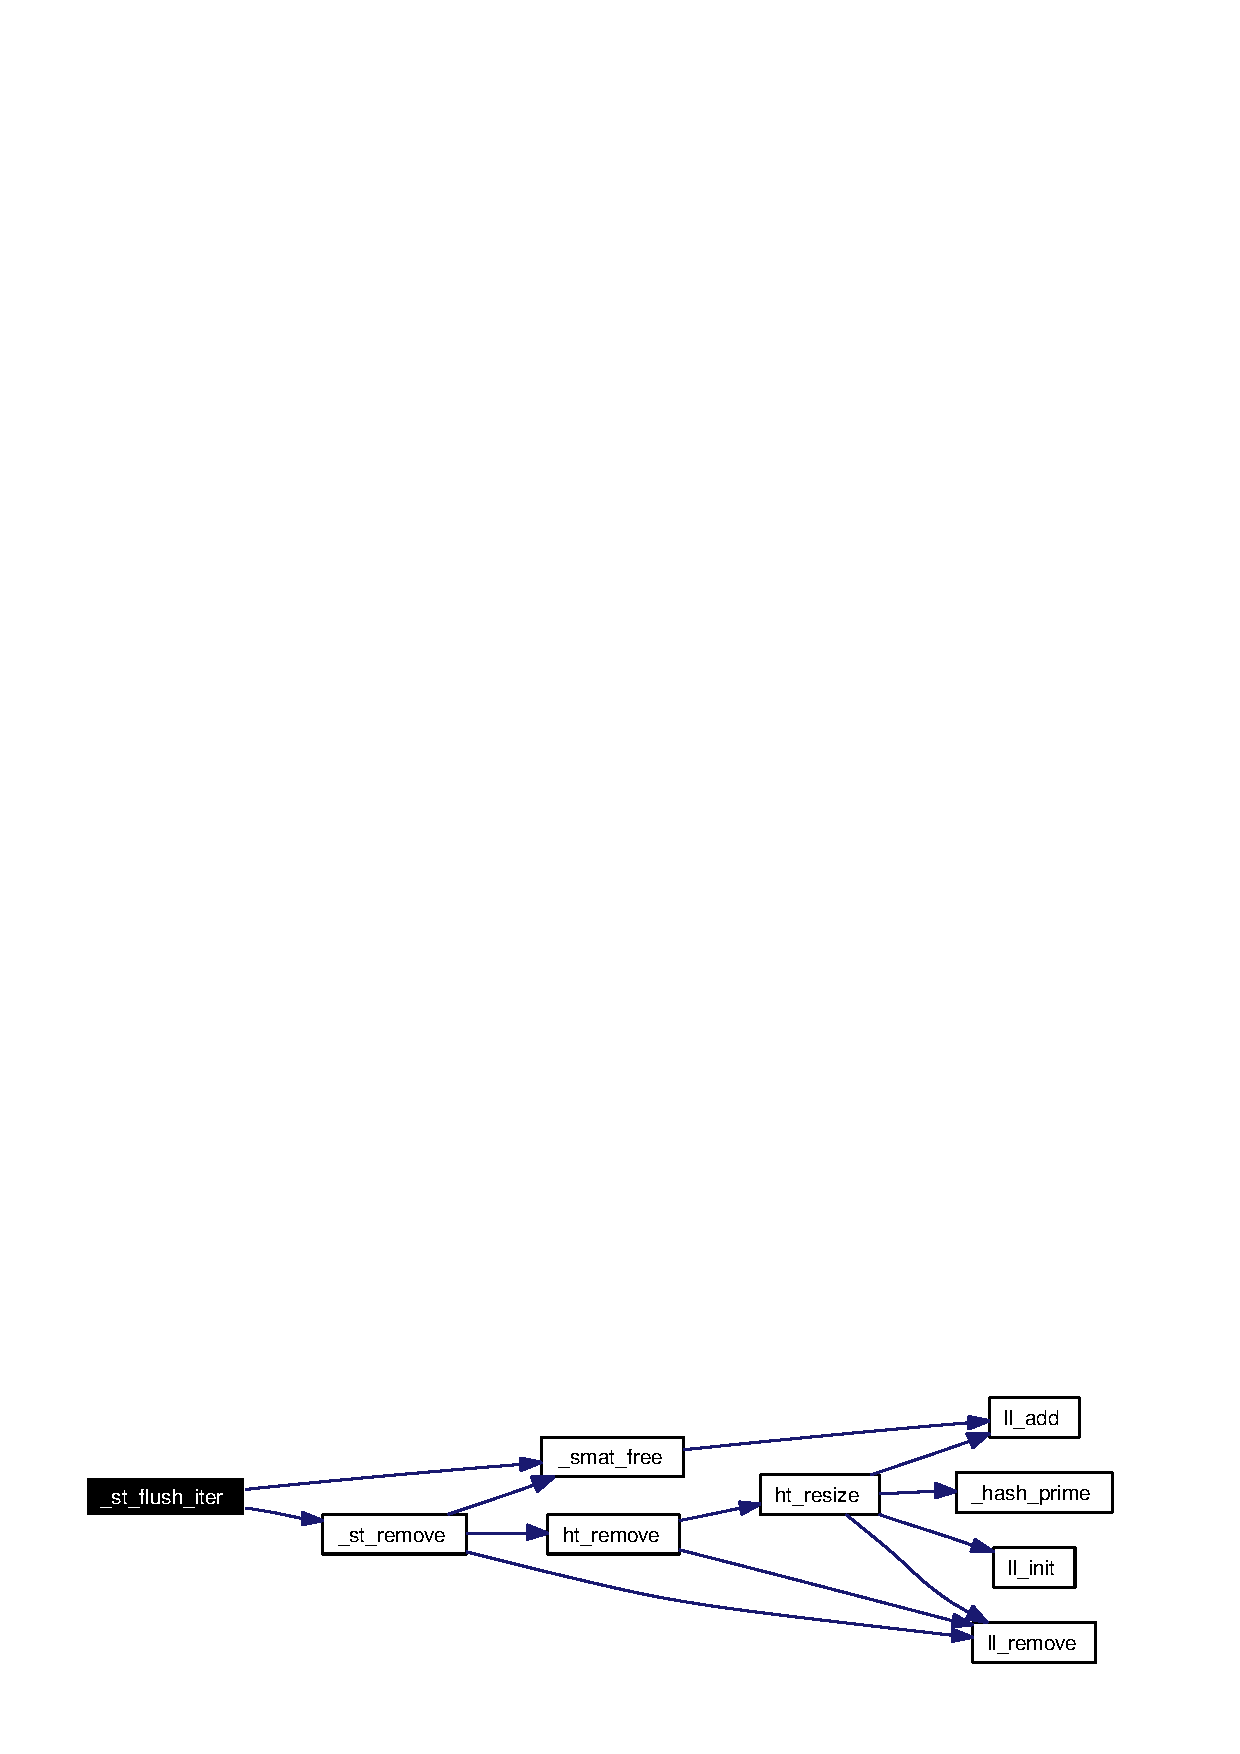
\includegraphics[width=269pt]{group__dbprim__smat_ga30_cgraph}
\end{center}
\end{figure}
\hypertarget{group__dbprim__smat_ga31}{
\index{dbprim_smat@{dbprim\_\-smat}!_st_iter_iter@{\_\-st\_\-iter\_\-iter}}
\index{_st_iter_iter@{\_\-st\_\-iter\_\-iter}!dbprim_smat@{dbprim\_\-smat}}
\subsubsection[\_\-st\_\-iter\_\-iter]{\setlength{\rightskip}{0pt plus 5cm}static unsigned long \_\-st\_\-iter\_\-iter (\hyperlink{struct__hash__table__s}{hash\_\-table\_\-t} $\ast$ {\em table}, \hyperlink{struct__hash__entry__s}{hash\_\-entry\_\-t} $\ast$ {\em ent}, void $\ast$ {\em extra})\hspace{0.3cm}{\tt  \mbox{[}static\mbox{]}}}}
\label{group__dbprim__smat_ga31}


\begin{Desc}
\item[For internal use only.]
This function is a \hyperlink{group__dbprim__hash_ga3}{hash\_\-iter\_\-t} iteration callback that is used as a shim between the \hyperlink{group__dbprim__smat_ga14}{st\_\-iter()} function and the \hyperlink{group__dbprim__hash_ga15}{ht\_\-iter()} function, which it uses internally.

\begin{Desc}
\item[Parameters:]
\begin{description}
\item[\mbox{$\leftarrow$} {\em table}]The hash table being iterated over. \item[\mbox{$\leftarrow$} {\em ent}]The specific hash table entry being processed. \item[\mbox{$\leftarrow$} {\em extra}]Extra caller-specific data to pass to the iteration function. In this case, a pointer to a struct \hyperlink{struct__st__iter__s}{\_\-st\_\-iter\_\-s} is passed.\end{description}
\end{Desc}
\begin{Desc}
\item[Returns:]Zero to continue iteration, non-zero otherwise.\end{Desc}
\end{Desc}


Definition at line 66 of file st\_\-iter.c.

References he\_\-value, \_\-st\_\-iter\_\-s::si\_\-extra, \_\-st\_\-iter\_\-s::si\_\-iter, and \_\-st\_\-iter\_\-s::si\_\-table.

Referenced by st\_\-iter().\hypertarget{group__dbprim__smat_ga23}{
\index{dbprim_smat@{dbprim\_\-smat}!_st_remove@{\_\-st\_\-remove}}
\index{_st_remove@{\_\-st\_\-remove}!dbprim_smat@{dbprim\_\-smat}}
\subsubsection[\_\-st\_\-remove]{\setlength{\rightskip}{0pt plus 5cm}unsigned long \_\-st\_\-remove (\hyperlink{struct__smat__table__s}{smat\_\-table\_\-t} $\ast$ {\em table}, \hyperlink{struct__smat__entry__s}{smat\_\-entry\_\-t} $\ast$ {\em entry}, unsigned int {\em remflag})}}
\label{group__dbprim__smat_ga23}


\begin{Desc}
\item[For internal use only.]
This function implements the actual logic that removes a sparse matrix entry from a sparse matrix table. Sparse matrix entries must be removed from three different locations before they can be passed to free(), and there are several places in the library where they are removed from one location and must subsequently be removed from the others. This routine allows the caller to specify exactly what must be removed through the use of the {\tt remflag} argument.

\begin{Desc}
\item[Parameters:]
\begin{description}
\item[\mbox{$\leftarrow$} {\em table}]A pointer to a \hyperlink{group__dbprim__smat_ga0}{smat\_\-table\_\-t}. \item[\mbox{$\leftarrow$} {\em entry}]A pointer to a \hyperlink{group__dbprim__smat_ga2}{smat\_\-entry\_\-t} to be removed from the table. \item[\mbox{$\leftarrow$} {\em remflag}]A bitwise mask of \hyperlink{group__dbprim__smat_ga66}{ST\_\-REM\_\-FIRST}, \hyperlink{group__dbprim__smat_ga67}{ST\_\-REM\_\-SECOND}, \hyperlink{group__dbprim__smat_ga68}{ST\_\-REM\_\-HASH}, and \hyperlink{group__dbprim__smat_ga69}{ST\_\-REM\_\-FREE} indicating which portions of the removal logic must be executed.\end{description}
\end{Desc}
\begin{Desc}
\item[Returns:]The function returns zero if the requested operations were completed successfully. A non-zero return value indicates a catastrophic failure condition, but is unlikely to occur.\end{Desc}
\end{Desc}


Definition at line 35 of file st\_\-remove.c.

References \_\-smat\_\-free(), ht\_\-remove(), ll\_\-remove(), \_\-smat\_\-entry\_\-s::se\_\-hash, \_\-smat\_\-entry\_\-s::se\_\-link, SMAT\_\-LOC\_\-FIRST, SMAT\_\-LOC\_\-SECOND, ST\_\-REM\_\-FIRST, ST\_\-REM\_\-FREE, ST\_\-REM\_\-HASH, ST\_\-REM\_\-SECOND, and \_\-smat\_\-table\_\-s::st\_\-table.

Referenced by \_\-sh\_\-flush\_\-iter(), \_\-st\_\-flush\_\-iter(), and st\_\-remove().

Here is the call graph for this function:\begin{figure}[H]
\begin{center}
\leavevmode
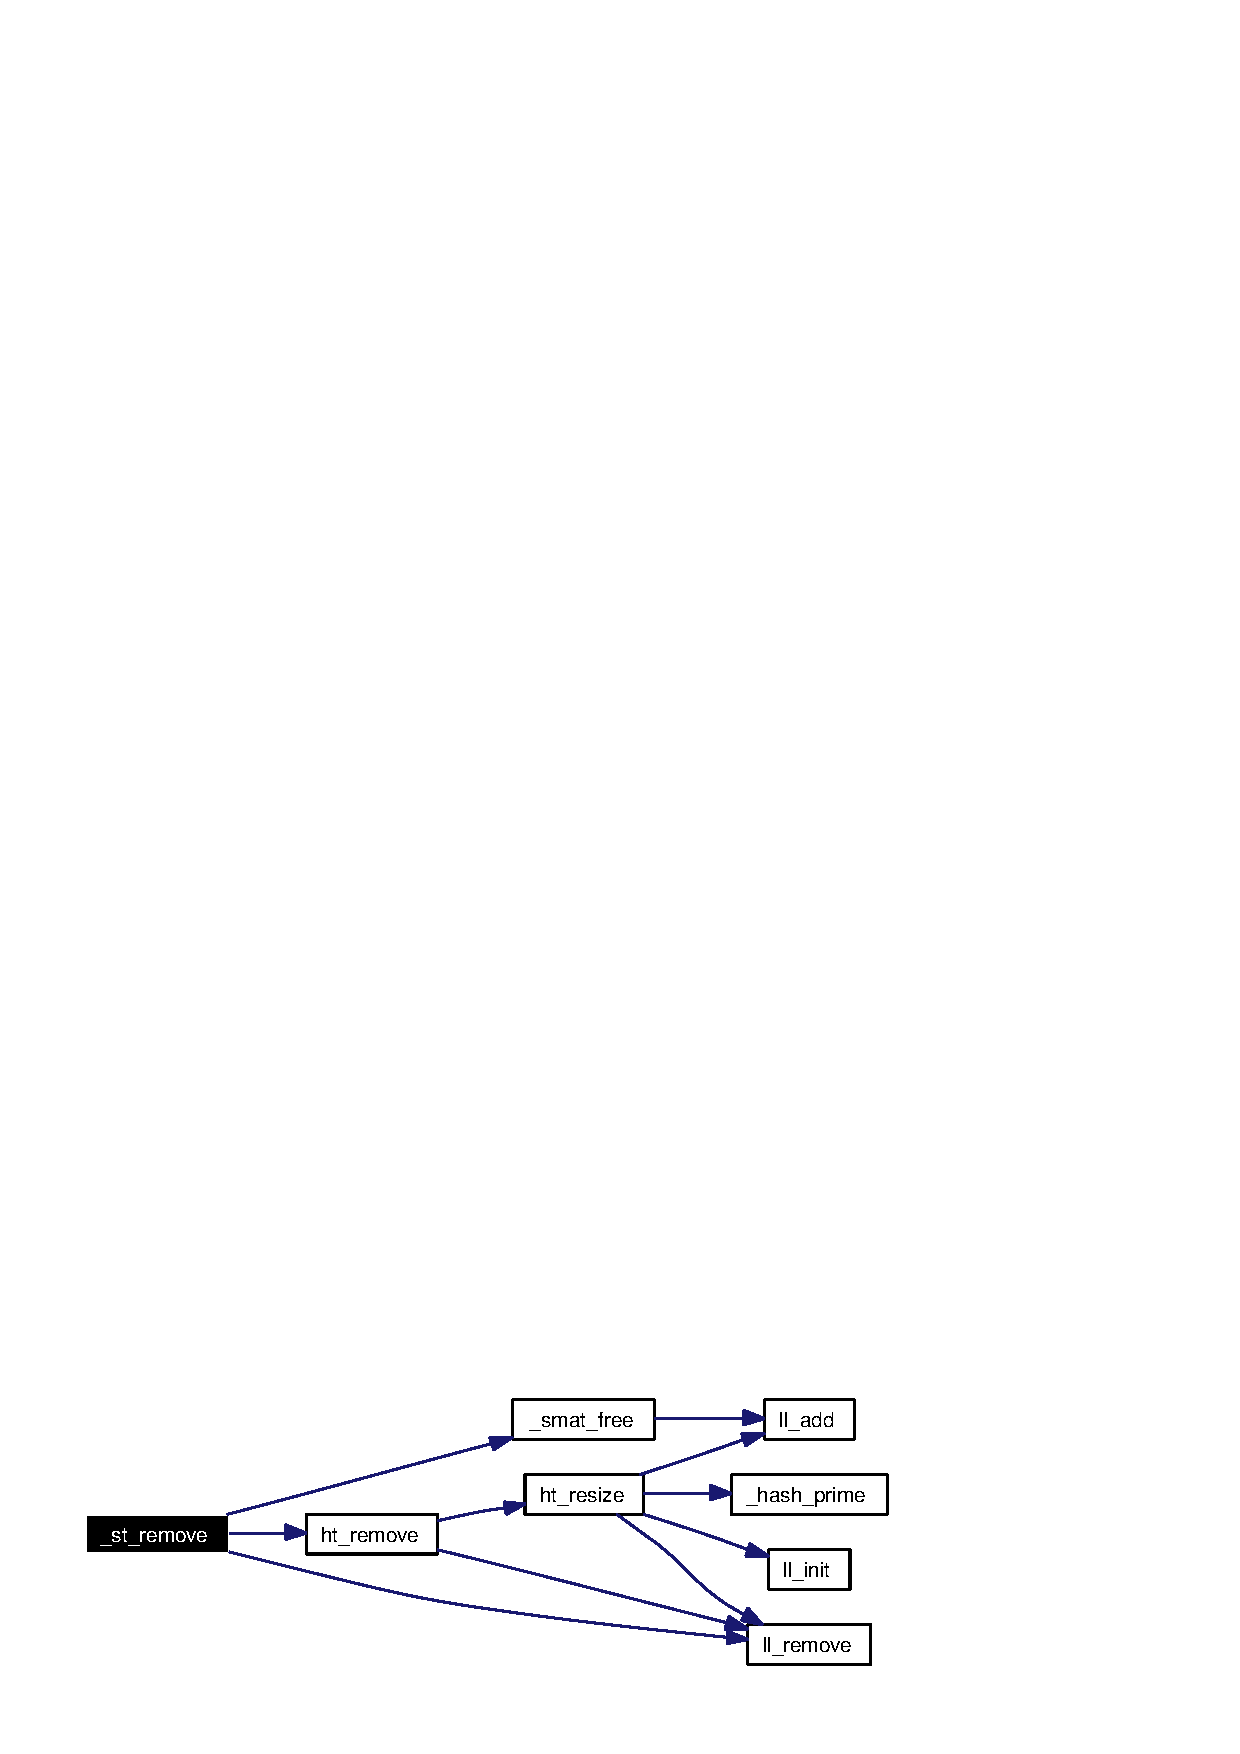
\includegraphics[width=215pt]{group__dbprim__smat_ga23_cgraph}
\end{center}
\end{figure}
\hypertarget{group__dbprim__smat_ga20}{
\index{dbprim_smat@{dbprim\_\-smat}!sh_find@{sh\_\-find}}
\index{sh_find@{sh\_\-find}!dbprim_smat@{dbprim\_\-smat}}
\subsubsection[sh\_\-find]{\setlength{\rightskip}{0pt plus 5cm}unsigned long sh\_\-find (\hyperlink{struct__smat__head__s}{smat\_\-head\_\-t} $\ast$ {\em head}, \hyperlink{struct__smat__entry__s}{smat\_\-entry\_\-t} $\ast$$\ast$ {\em elem\_\-p}, \hyperlink{group__dbprim__smat_ga5}{smat\_\-comp\_\-t} {\em comp\_\-func}, \hyperlink{struct__smat__entry__s}{smat\_\-entry\_\-t} $\ast$ {\em start}, \hyperlink{struct__db__key__s}{db\_\-key\_\-t} $\ast$ {\em key})}}
\label{group__dbprim__smat_ga20}


This function iterates through the given row or column of a sparse matrix looking for an element that matches the given {\tt key}.

\begin{Desc}
\item[Parameters:]
\begin{description}
\item[\mbox{$\leftarrow$} {\em head}]A pointer to a \hyperlink{group__dbprim__smat_ga1}{smat\_\-head\_\-t}. \item[\mbox{$\rightarrow$} {\em elem\_\-p}]A pointer to a pointer to a \hyperlink{group__dbprim__smat_ga2}{smat\_\-entry\_\-t}. {\tt NULL} is an invalid value. \item[\mbox{$\leftarrow$} {\em comp\_\-func}]A pointer to a comparison function used to compare the key to a particular entry. See the documentation for \hyperlink{group__dbprim__smat_ga5}{smat\_\-comp\_\-t} for more information. \item[\mbox{$\leftarrow$} {\em start}]A pointer to a \hyperlink{group__dbprim__smat_ga2}{smat\_\-entry\_\-t} describing where in the row or column to start. If {\tt NULL} is passed, the beginning of the row or column will be assumed. \item[\mbox{$\leftarrow$} {\em key}]A key to search for.\end{description}
\end{Desc}
\begin{Desc}
\item[Return values:]
\begin{description}
\item[{\em DB\_\-ERR\_\-BADARGS}]An argument was invalid. \item[{\em DB\_\-ERR\_\-WRONGTABLE}]{\tt start} is not in this row or column. \item[{\em DB\_\-ERR\_\-NOENTRY}]No matching entry was found.\end{description}
\end{Desc}


Definition at line 72 of file sh\_\-find.c.

References \_\-sh\_\-find\_\-comp(), dk\_\-key, le\_\-object, ll\_\-find(), \_\-smat\_\-entry\_\-s::se\_\-link, se\_\-verify, \_\-sh\_\-find\_\-s::sf\_\-comp, \_\-sh\_\-find\_\-s::sf\_\-key, \_\-smat\_\-head\_\-s::sh\_\-elem, \_\-smat\_\-head\_\-s::sh\_\-head, and sh\_\-verify.

Here is the call graph for this function:\begin{figure}[H]
\begin{center}
\leavevmode
\includegraphics[width=108pt]{group__dbprim__smat_ga20_cgraph}
\end{center}
\end{figure}
\hypertarget{group__dbprim__smat_ga22}{
\index{dbprim_smat@{dbprim\_\-smat}!sh_flush@{sh\_\-flush}}
\index{sh_flush@{sh\_\-flush}!dbprim_smat@{dbprim\_\-smat}}
\subsubsection[sh\_\-flush]{\setlength{\rightskip}{0pt plus 5cm}unsigned long sh\_\-flush (\hyperlink{struct__smat__head__s}{smat\_\-head\_\-t} $\ast$ {\em head}, \hyperlink{group__dbprim__smat_ga4}{smat\_\-iter\_\-t} {\em flush\_\-func}, void $\ast$ {\em extra})}}
\label{group__dbprim__smat_ga22}


This function flushes a sparse matrix row or column--that is, it removes each element from that row or column. If a {\tt flush\_\-func} is specified, it will be called on the entry after it has been removed from the row or column, and may safely call {\tt free()}.

\begin{Desc}
\item[Parameters:]
\begin{description}
\item[\mbox{$\leftarrow$} {\em head}]A pointer to a \hyperlink{group__dbprim__smat_ga1}{smat\_\-head\_\-t}. \item[\mbox{$\leftarrow$} {\em flush\_\-func}]A pointer to a callback function used to perform user-specifed actions on an entry after removing it from the row or column. May be {\tt NULL}. See the documentation for \hyperlink{group__dbprim__smat_ga4}{smat\_\-iter\_\-t} for more information. \item[\mbox{$\leftarrow$} {\em extra}]A {\tt void} pointer that will be passed to {\tt flush\_\-func}.\end{description}
\end{Desc}
\begin{Desc}
\item[Return values:]
\begin{description}
\item[{\em DB\_\-ERR\_\-BADARGS}]An argument was invalid.\end{description}
\end{Desc}


Definition at line 90 of file sh\_\-flush.c.

References \_\-sh\_\-flush\_\-iter(), ll\_\-flush(), \_\-sh\_\-flush\_\-s::sf\_\-elem, \_\-sh\_\-flush\_\-s::sf\_\-extra, \_\-sh\_\-flush\_\-s::sf\_\-flush, \_\-sh\_\-flush\_\-s::sf\_\-table, \_\-smat\_\-head\_\-s::sh\_\-elem, \_\-smat\_\-head\_\-s::sh\_\-head, \_\-smat\_\-head\_\-s::sh\_\-table, and sh\_\-verify.

Here is the call graph for this function:\begin{figure}[H]
\begin{center}
\leavevmode
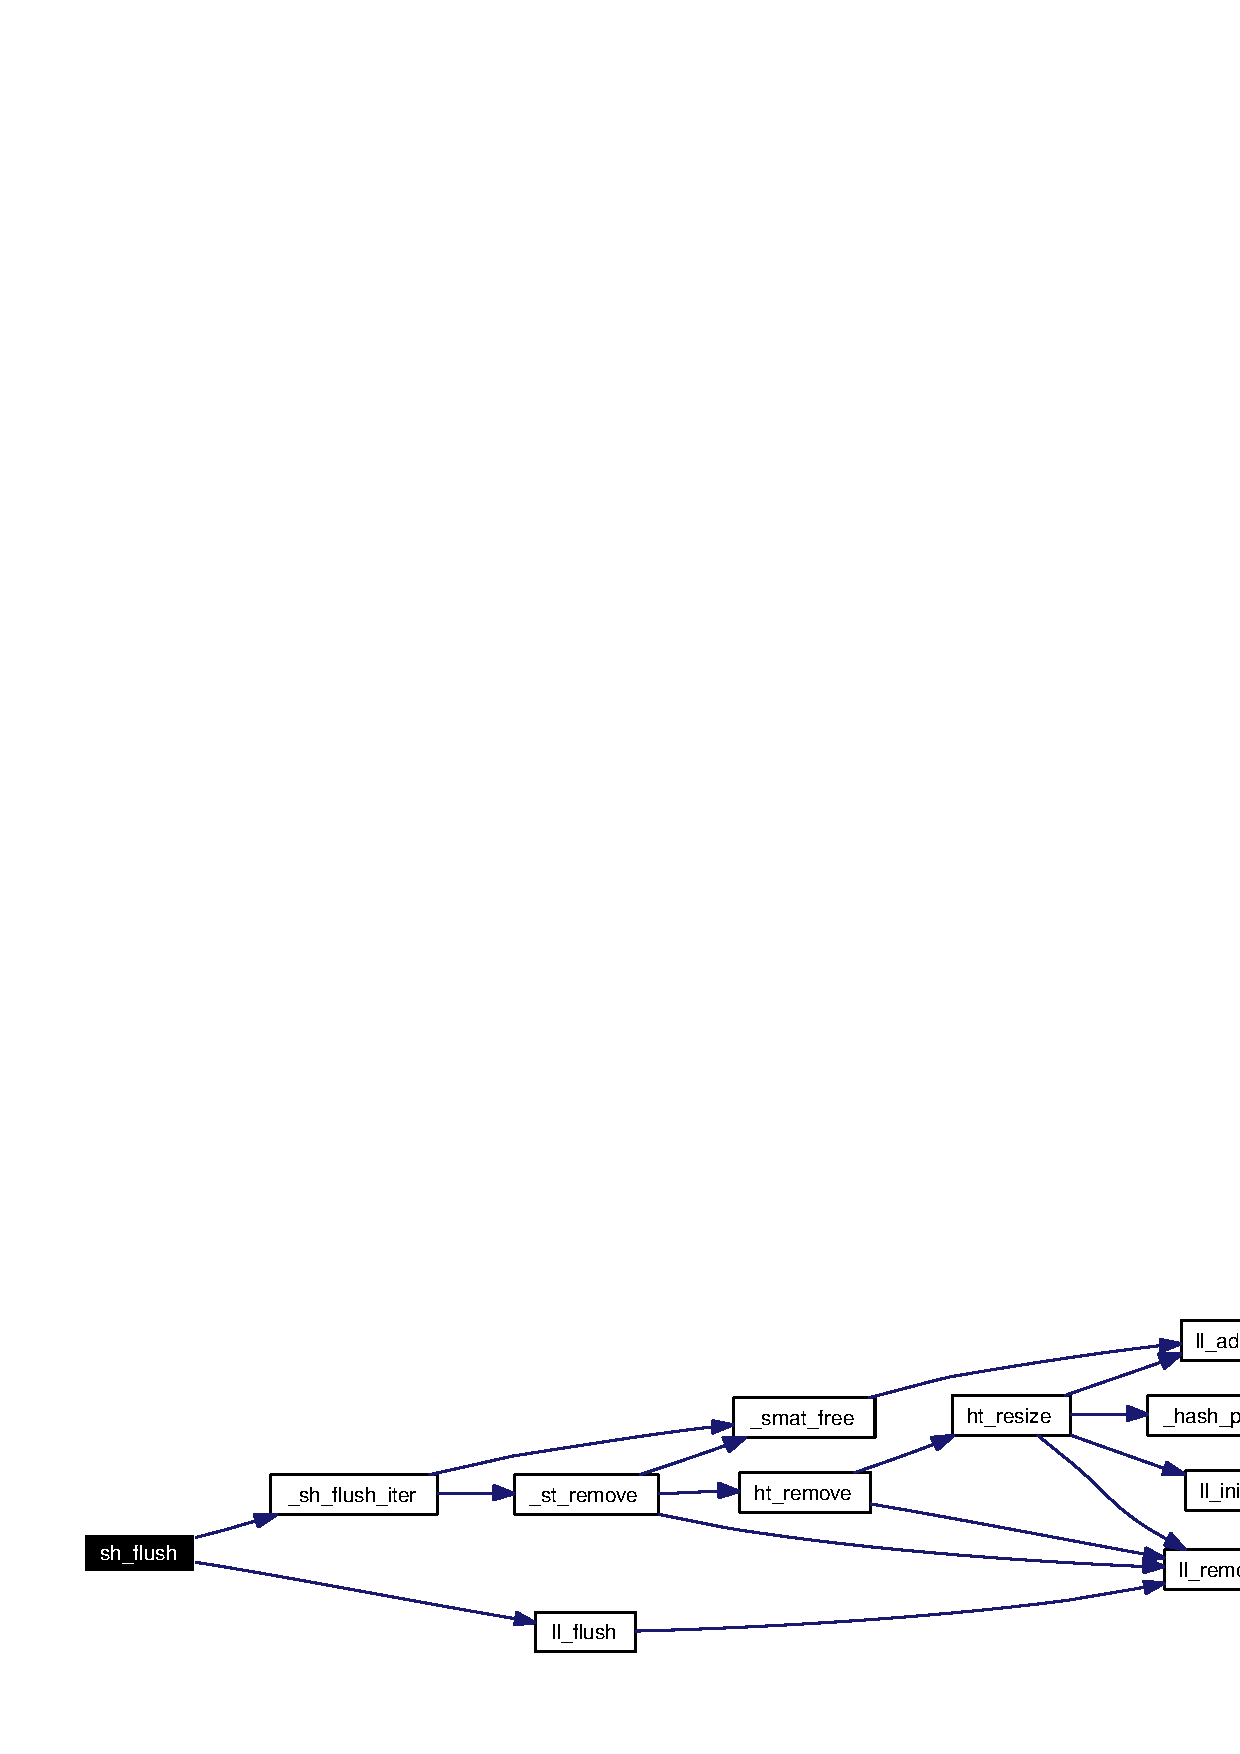
\includegraphics[width=315pt]{group__dbprim__smat_ga22_cgraph}
\end{center}
\end{figure}
\hypertarget{group__dbprim__smat_ga18}{
\index{dbprim_smat@{dbprim\_\-smat}!sh_init@{sh\_\-init}}
\index{sh_init@{sh\_\-init}!dbprim_smat@{dbprim\_\-smat}}
\subsubsection[sh\_\-init]{\setlength{\rightskip}{0pt plus 5cm}unsigned long sh\_\-init (\hyperlink{struct__smat__head__s}{smat\_\-head\_\-t} $\ast$ {\em head}, \hyperlink{group__dbprim__smat_ga6}{smat\_\-loc\_\-t} {\em elem}, void $\ast$ {\em object})}}
\label{group__dbprim__smat_ga18}


This function dynamically initializes a sparse matrix row or column linked list head. The {\tt elem} argument specifies whether the object is to be associated with a \hyperlink{group__dbprim__smat_gga70a137}{SMAT\_\-LOC\_\-FIRST} list or a \hyperlink{group__dbprim__smat_gga70a138}{SMAT\_\-LOC\_\-SECOND} list.

\begin{Desc}
\item[Parameters:]
\begin{description}
\item[\mbox{$\leftarrow$} {\em head}]A pointer to a \hyperlink{group__dbprim__smat_ga1}{smat\_\-head\_\-t} to be initialized. \item[\mbox{$\leftarrow$} {\em elem}]Either \hyperlink{group__dbprim__smat_gga70a137}{SMAT\_\-LOC\_\-FIRST} or \hyperlink{group__dbprim__smat_gga70a138}{SMAT\_\-LOC\_\-SECOND}. \item[\mbox{$\leftarrow$} {\em object}]A pointer to the object containing the sparse matrix row or column head.\end{description}
\end{Desc}
\begin{Desc}
\item[Return values:]
\begin{description}
\item[{\em DB\_\-ERR\_\-BADARGS}]An invalid argument was given.\end{description}
\end{Desc}


Definition at line 34 of file sh\_\-init.c.

References ll\_\-init(), \_\-smat\_\-head\_\-s::sh\_\-elem, \_\-smat\_\-head\_\-s::sh\_\-head, \_\-smat\_\-head\_\-s::sh\_\-magic, \_\-smat\_\-head\_\-s::sh\_\-table, SMAT\_\-HEAD\_\-MAGIC, SMAT\_\-LOC\_\-FIRST, and SMAT\_\-LOC\_\-SECOND.

Here is the call graph for this function:\begin{figure}[H]
\begin{center}
\leavevmode
\includegraphics[width=83pt]{group__dbprim__smat_ga18_cgraph}
\end{center}
\end{figure}
\hypertarget{group__dbprim__smat_ga21}{
\index{dbprim_smat@{dbprim\_\-smat}!sh_iter@{sh\_\-iter}}
\index{sh_iter@{sh\_\-iter}!dbprim_smat@{dbprim\_\-smat}}
\subsubsection[sh\_\-iter]{\setlength{\rightskip}{0pt plus 5cm}unsigned long sh\_\-iter (\hyperlink{struct__smat__head__s}{smat\_\-head\_\-t} $\ast$ {\em head}, \hyperlink{struct__smat__entry__s}{smat\_\-entry\_\-t} $\ast$ {\em start}, \hyperlink{group__dbprim__smat_ga4}{smat\_\-iter\_\-t} {\em iter\_\-func}, void $\ast$ {\em extra}, unsigned long {\em flags})}}
\label{group__dbprim__smat_ga21}


This function iterates over a row or column of a sparse matrix, executing the given {\tt iter\_\-func} for each entry.

\begin{Desc}
\item[Parameters:]
\begin{description}
\item[\mbox{$\leftarrow$} {\em head}]A pointer to a \hyperlink{group__dbprim__smat_ga1}{smat\_\-head\_\-t}. \item[\mbox{$\leftarrow$} {\em start}]A pointer to a \hyperlink{group__dbprim__smat_ga2}{smat\_\-entry\_\-t} describing where in the row or column to start. If {\tt NULL} is passed, the beginning of the row or column will be assumed. \item[\mbox{$\leftarrow$} {\em iter\_\-func}]A pointer to a callback function used to perform user-specified actions on an entry in a row or column of a sparse matrix. {\tt NULL} is an invalid value. See the documentation for \hyperlink{group__dbprim__smat_ga4}{smat\_\-iter\_\-t} for more information. \item[\mbox{$\leftarrow$} {\em extra}]A {\tt void} pointer that will be passed to {\tt iter\_\-func}. \item[\mbox{$\leftarrow$} {\em flags}]If \hyperlink{group__dbprim_ga4}{DB\_\-FLAG\_\-REVERSE} is given, iteration will be done from the end of the list backwards towards the head.\end{description}
\end{Desc}
\begin{Desc}
\item[Return values:]
\begin{description}
\item[{\em DB\_\-ERR\_\-BADARGS}]An argument was invalid. \item[{\em DB\_\-ERR\_\-WRONGTABLE}]{\tt start} is not in this row or column.\end{description}
\end{Desc}


Definition at line 77 of file sh\_\-iter.c.

References \_\-sh\_\-iter\_\-iter(), ll\_\-iter(), \_\-smat\_\-entry\_\-s::se\_\-link, se\_\-verify, \_\-smat\_\-head\_\-s::sh\_\-elem, \_\-smat\_\-head\_\-s::sh\_\-head, \_\-smat\_\-head\_\-s::sh\_\-table, sh\_\-verify, \_\-sh\_\-iter\_\-s::si\_\-extra, \_\-sh\_\-iter\_\-s::si\_\-iter, and \_\-sh\_\-iter\_\-s::si\_\-table.

Here is the call graph for this function:\begin{figure}[H]
\begin{center}
\leavevmode
\includegraphics[width=99pt]{group__dbprim__smat_ga21_cgraph}
\end{center}
\end{figure}
\hypertarget{group__dbprim__smat_ga19}{
\index{dbprim_smat@{dbprim\_\-smat}!sh_move@{sh\_\-move}}
\index{sh_move@{sh\_\-move}!dbprim_smat@{dbprim\_\-smat}}
\subsubsection[sh\_\-move]{\setlength{\rightskip}{0pt plus 5cm}unsigned long sh\_\-move (\hyperlink{struct__smat__head__s}{smat\_\-head\_\-t} $\ast$ {\em head}, \hyperlink{struct__smat__entry__s}{smat\_\-entry\_\-t} $\ast$ {\em elem}, \hyperlink{group__dbprim__link_ga4}{link\_\-loc\_\-t} {\em loc}, \hyperlink{struct__smat__entry__s}{smat\_\-entry\_\-t} $\ast$ {\em elem2})}}
\label{group__dbprim__smat_ga19}


This function allows the specified entry to be shifted within the linked list describing the row or column. It is very similar to the \hyperlink{group__dbprim__link_ga7}{ll\_\-move()} function.

\begin{Desc}
\item[Parameters:]
\begin{description}
\item[\mbox{$\leftarrow$} {\em head}]A pointer to a \hyperlink{group__dbprim__smat_ga1}{smat\_\-head\_\-t}. \item[\mbox{$\leftarrow$} {\em elem}]A pointer to the \hyperlink{group__dbprim__smat_ga2}{smat\_\-entry\_\-t} describing the entry to be moved. \item[\mbox{$\leftarrow$} {\em loc}]A \hyperlink{group__dbprim__link_ga4}{link\_\-loc\_\-t} indicating where the entry should be moved to. \item[\mbox{$\leftarrow$} {\em elem2}]A pointer to a \hyperlink{group__dbprim__smat_ga2}{smat\_\-entry\_\-t} describing another entry in the list if {\tt loc} is \hyperlink{group__dbprim__link_gga28a135}{LINK\_\-LOC\_\-BEFORE} or \hyperlink{group__dbprim__link_gga28a136}{LINK\_\-LOC\_\-AFTER}.\end{description}
\end{Desc}
\begin{Desc}
\item[Return values:]
\begin{description}
\item[{\em DB\_\-ERR\_\-BADARGS}]An argument was invalid. \item[{\em DB\_\-ERR\_\-BUSY}]{\tt elem} and {\tt elem2} are the same entry. \item[{\em DB\_\-ERR\_\-WRONGTABLE}]{\tt elem} or {\tt elem2} are in a different row or column. \item[{\em DB\_\-ERR\_\-UNUSED}]{\tt elem} or {\tt elem2} are not in any row or column.\end{description}
\end{Desc}


Definition at line 35 of file sh\_\-move.c.

References ll\_\-move(), \_\-smat\_\-entry\_\-s::se\_\-link, se\_\-verify, \_\-smat\_\-head\_\-s::sh\_\-elem, \_\-smat\_\-head\_\-s::sh\_\-head, and sh\_\-verify.

Here is the call graph for this function:\begin{figure}[H]
\begin{center}
\leavevmode
\includegraphics[width=94pt]{group__dbprim__smat_ga19_cgraph}
\end{center}
\end{figure}
\hypertarget{group__dbprim__smat_ga8}{
\index{dbprim_smat@{dbprim\_\-smat}!smat_cleanup@{smat\_\-cleanup}}
\index{smat_cleanup@{smat\_\-cleanup}!dbprim_smat@{dbprim\_\-smat}}
\subsubsection[smat\_\-cleanup]{\setlength{\rightskip}{0pt plus 5cm}unsigned long smat\_\-cleanup (void)}}
\label{group__dbprim__smat_ga8}


This function frees all smat\_\-entry\_\-t objects on the internal free list. It is always successful and returns 0.

\begin{Desc}
\item[Returns:]This function always returns 0.\end{Desc}


Definition at line 90 of file smat\_\-freelist.c.

References le\_\-object, ll\_\-first, and ll\_\-remove().

Here is the call graph for this function:\begin{figure}[H]
\begin{center}
\leavevmode
\includegraphics[width=110pt]{group__dbprim__smat_ga8_cgraph}
\end{center}
\end{figure}
\hypertarget{group__dbprim__smat_ga9}{
\index{dbprim_smat@{dbprim\_\-smat}!smat_freemem@{smat\_\-freemem}}
\index{smat_freemem@{smat\_\-freemem}!dbprim_smat@{dbprim\_\-smat}}
\subsubsection[smat\_\-freemem]{\setlength{\rightskip}{0pt plus 5cm}unsigned long smat\_\-freemem (void)}}
\label{group__dbprim__smat_ga9}


This function returns the amount of memory being used by the internal free list of smat\_\-entry\_\-t objects.

\begin{Desc}
\item[Returns:]A number indicating the size, in bytes, of the memory allocated for smat\_\-entry\_\-t objects on the free list.\end{Desc}


Definition at line 106 of file smat\_\-freelist.c.

References ll\_\-count.\hypertarget{group__dbprim__smat_ga11}{
\index{dbprim_smat@{dbprim\_\-smat}!st_add@{st\_\-add}}
\index{st_add@{st\_\-add}!dbprim_smat@{dbprim\_\-smat}}
\subsubsection[st\_\-add]{\setlength{\rightskip}{0pt plus 5cm}unsigned long st\_\-add (\hyperlink{struct__smat__table__s}{smat\_\-table\_\-t} $\ast$ {\em table}, \hyperlink{struct__smat__entry__s}{smat\_\-entry\_\-t} $\ast$$\ast$ {\em entry\_\-p}, \hyperlink{struct__smat__head__s}{smat\_\-head\_\-t} $\ast$ {\em head1}, \hyperlink{group__dbprim__link_ga4}{link\_\-loc\_\-t} {\em loc1}, \hyperlink{struct__smat__entry__s}{smat\_\-entry\_\-t} $\ast$ {\em ent1}, \hyperlink{struct__smat__head__s}{smat\_\-head\_\-t} $\ast$ {\em head2}, \hyperlink{group__dbprim__link_ga4}{link\_\-loc\_\-t} {\em loc2}, \hyperlink{struct__smat__entry__s}{smat\_\-entry\_\-t} $\ast$ {\em ent2})}}
\label{group__dbprim__smat_ga11}


This function adds an entry to a sparse matrix. The entry is referenced in three different places, thus the complex set of arguments. This function will allocate a \hyperlink{group__dbprim__smat_ga2}{smat\_\-entry\_\-t} and return it through the {\tt entry\_\-p} result parameter.

\begin{Desc}
\item[Parameters:]
\begin{description}
\item[\mbox{$\leftarrow$} {\em table}]A pointer to a \hyperlink{group__dbprim__smat_ga0}{smat\_\-table\_\-t}. \item[\mbox{$\rightarrow$} {\em entry\_\-p}]A pointer to a pointer to a \hyperlink{group__dbprim__smat_ga2}{smat\_\-entry\_\-t}. If {\tt NULL} is passed, the addition will be performed and an appropriate error code returned. \item[\mbox{$\leftarrow$} {\em head1}]A pointer to a \hyperlink{group__dbprim__smat_ga1}{smat\_\-head\_\-t} representing a \hyperlink{group__dbprim__smat_gga70a137}{SMAT\_\-LOC\_\-FIRST} sparse matrix list. \item[\mbox{$\leftarrow$} {\em loc1}]A \hyperlink{group__dbprim__link_ga4}{link\_\-loc\_\-t} indicating where the entry should be added for {\tt head1}. \item[\mbox{$\leftarrow$} {\em ent1}]A pointer to a \hyperlink{group__dbprim__smat_ga2}{smat\_\-entry\_\-t} describing another element in the list represented by {\tt head1} if {\tt loc1} is \hyperlink{group__dbprim__link_gga28a135}{LINK\_\-LOC\_\-BEFORE} or \hyperlink{group__dbprim__link_gga28a136}{LINK\_\-LOC\_\-AFTER}. \item[\mbox{$\leftarrow$} {\em head2}]A pointer to a \hyperlink{group__dbprim__smat_ga1}{smat\_\-head\_\-t} representing a \hyperlink{group__dbprim__smat_gga70a138}{SMAT\_\-LOC\_\-SECOND} sparse matrix list. \item[\mbox{$\leftarrow$} {\em loc2}]A \hyperlink{group__dbprim__link_ga4}{link\_\-loc\_\-t} indicating where the entry should be added for {\tt head2}. \item[\mbox{$\leftarrow$} {\em ent2}]A pointer to a \hyperlink{group__dbprim__smat_ga2}{smat\_\-entry\_\-t} describing another element in the list represented by {\tt head2} if {\tt loc2} is \hyperlink{group__dbprim__link_gga28a135}{LINK\_\-LOC\_\-BEFORE} or \hyperlink{group__dbprim__link_gga28a136}{LINK\_\-LOC\_\-AFTER}.\end{description}
\end{Desc}
\begin{Desc}
\item[Return values:]
\begin{description}
\item[{\em DB\_\-ERR\_\-BADARGS}]An argument was invalid. \item[{\em DB\_\-ERR\_\-BUSY}]One of the arguments is already in the table. \item[{\em DB\_\-ERR\_\-FROZEN}]The table is currently frozen. \item[{\em DB\_\-ERR\_\-NOTABLE}]The bucket table has not been allocated and automatic growth is not enabled. \item[{\em DB\_\-ERR\_\-WRONGTABLE}]One of the arguments was not in the proper table or list. \item[{\em DB\_\-ERR\_\-UNUSED}]One of the {\tt ent} arguments is not presently in a list. \item[{\em DB\_\-ERR\_\-UNRECOVERABLE}]An unrecoverable error occurred while resizing the table. \item[{\em ENOMEM}]No memory could be allocated for the \hyperlink{group__dbprim__smat_ga2}{smat\_\-entry\_\-t} structure.\end{description}
\end{Desc}


Definition at line 36 of file st\_\-add.c.

References \_\-smat\_\-alloc(), \_\-smat\_\-free(), dk\_\-key, dk\_\-len, ht\_\-add(), ht\_\-remove(), LINK\_\-LOC\_\-AFTER, LINK\_\-LOC\_\-BEFORE, ll\_\-add(), ll\_\-remove(), \_\-smat\_\-entry\_\-s::se\_\-hash, \_\-smat\_\-entry\_\-s::se\_\-link, \_\-smat\_\-entry\_\-s::se\_\-object, \_\-smat\_\-entry\_\-s::se\_\-table, se\_\-verify, \_\-smat\_\-head\_\-s::sh\_\-elem, \_\-smat\_\-head\_\-s::sh\_\-head, sh\_\-object, \_\-smat\_\-head\_\-s::sh\_\-table, sh\_\-verify, SMAT\_\-LOC\_\-FIRST, SMAT\_\-LOC\_\-SECOND, ST\_\-REM\_\-FIRST, ST\_\-REM\_\-FREE, ST\_\-REM\_\-HASH, \_\-smat\_\-table\_\-s::st\_\-table, and st\_\-verify.

Here is the call graph for this function:\begin{figure}[H]
\begin{center}
\leavevmode
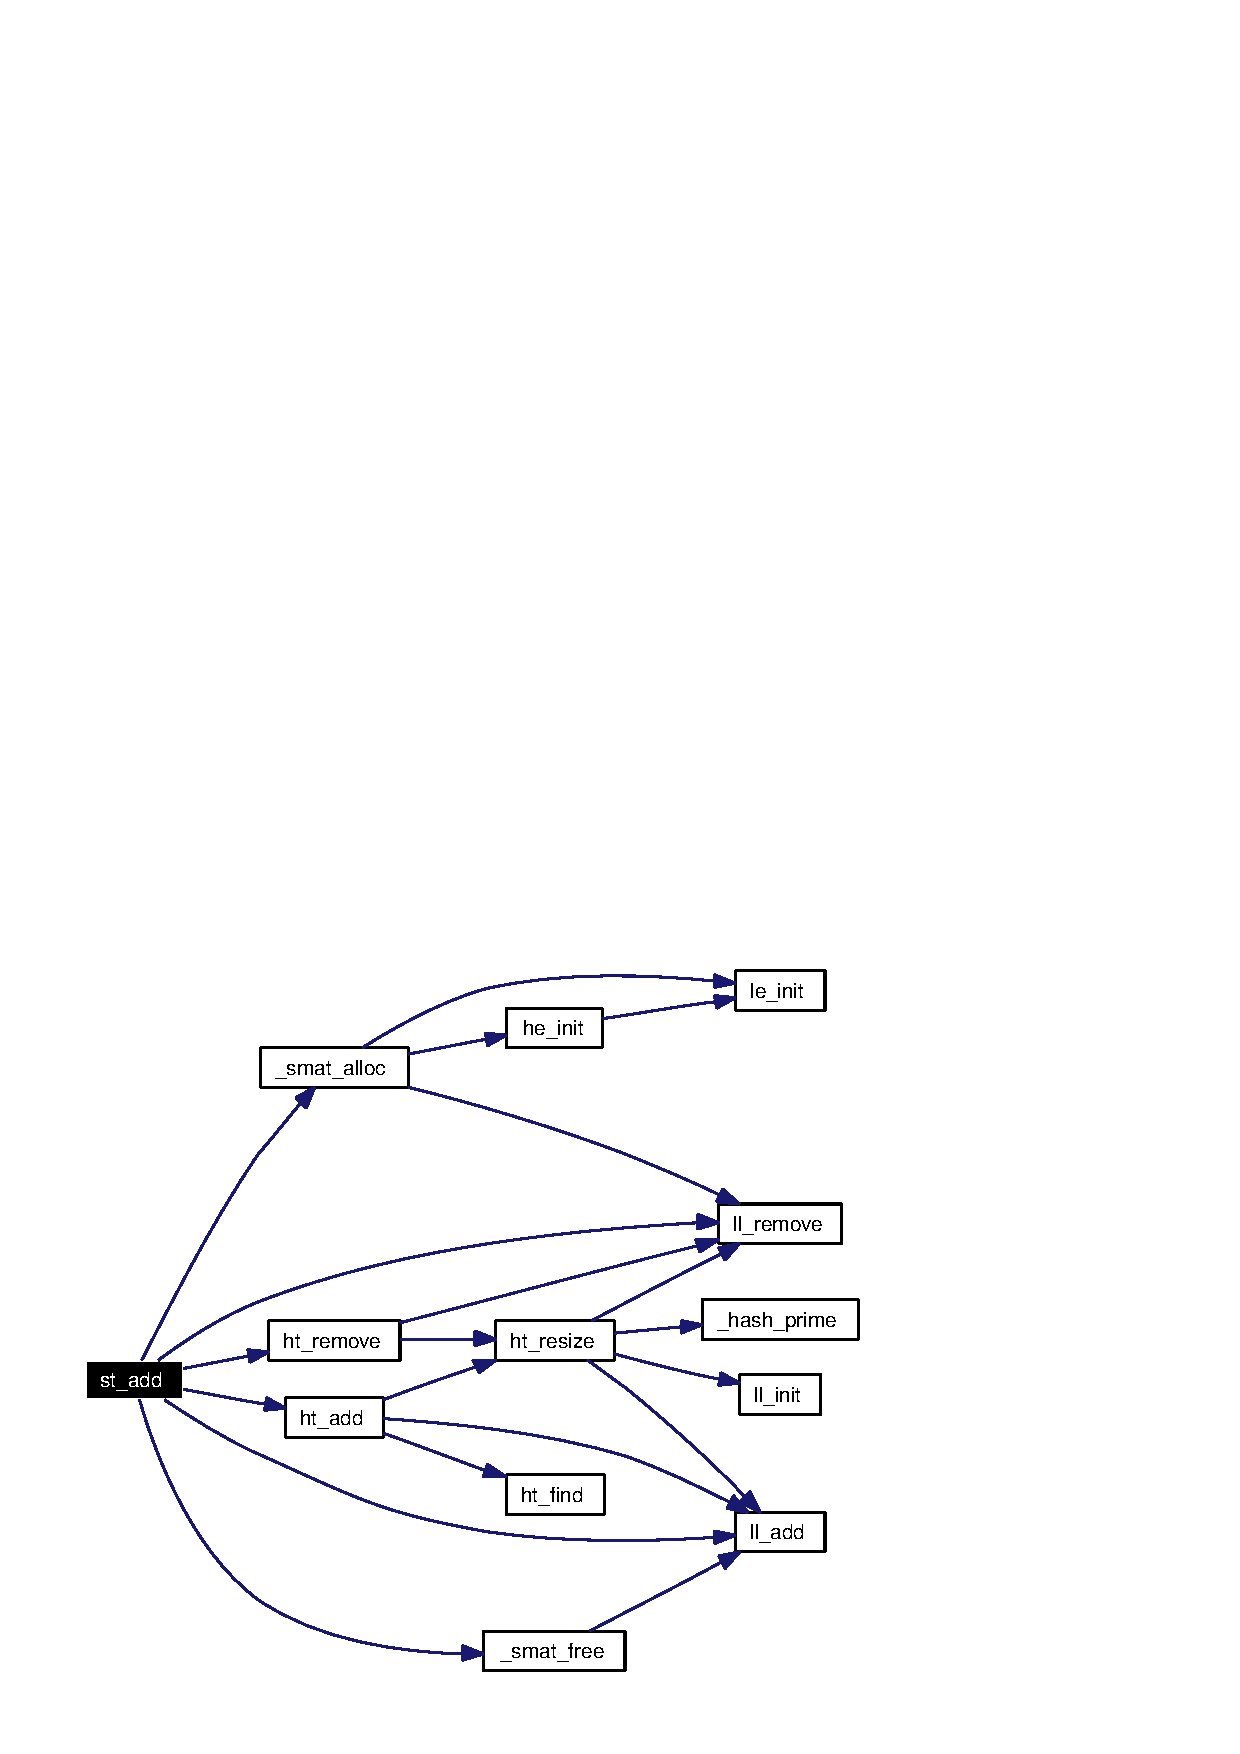
\includegraphics[width=208pt]{group__dbprim__smat_ga11_cgraph}
\end{center}
\end{figure}
\hypertarget{group__dbprim__smat_ga13}{
\index{dbprim_smat@{dbprim\_\-smat}!st_find@{st\_\-find}}
\index{st_find@{st\_\-find}!dbprim_smat@{dbprim\_\-smat}}
\subsubsection[st\_\-find]{\setlength{\rightskip}{0pt plus 5cm}unsigned long st\_\-find (\hyperlink{struct__smat__table__s}{smat\_\-table\_\-t} $\ast$ {\em table}, \hyperlink{struct__smat__entry__s}{smat\_\-entry\_\-t} $\ast$$\ast$ {\em entry\_\-p}, \hyperlink{struct__smat__head__s}{smat\_\-head\_\-t} $\ast$ {\em head1}, \hyperlink{struct__smat__head__s}{smat\_\-head\_\-t} $\ast$ {\em head2})}}
\label{group__dbprim__smat_ga13}


This function looks up the entry matching the given {\tt head1} and {\tt head2}.

\begin{Desc}
\item[Parameters:]
\begin{description}
\item[\mbox{$\leftarrow$} {\em table}]A pointer to a \hyperlink{group__dbprim__smat_ga0}{smat\_\-table\_\-t}. \item[\mbox{$\rightarrow$} {\em entry\_\-p}]A pointer to a pointer to a \hyperlink{group__dbprim__smat_ga2}{smat\_\-entry\_\-t}. If {\tt NULL} is passed, the lookup will be performed and an appropriate error code returned. \item[\mbox{$\leftarrow$} {\em head1}]A pointer to a \hyperlink{group__dbprim__smat_ga1}{smat\_\-head\_\-t} initialized to \hyperlink{group__dbprim__smat_gga70a137}{SMAT\_\-LOC\_\-FIRST}. \item[\mbox{$\leftarrow$} {\em head2}]A pointer to a \hyperlink{group__dbprim__smat_ga1}{smat\_\-head\_\-t} initialized to \hyperlink{group__dbprim__smat_gga70a138}{SMAT\_\-LOC\_\-SECOND}.\end{description}
\end{Desc}
\begin{Desc}
\item[Return values:]
\begin{description}
\item[{\em DB\_\-ERR\_\-BADARGS}]An argument was invalid. \item[{\em DB\_\-ERR\_\-WRONGTABLE}]One or both of {\tt head1} or {\tt head2} are not referenced in this table. \item[{\em DB\_\-ERR\_\-NOENTRY}]No matching entry was found.\end{description}
\end{Desc}


Definition at line 36 of file st\_\-find.c.

References dk\_\-key, dk\_\-len, he\_\-value, ht\_\-find(), \_\-link\_\-head\_\-s::lh\_\-count, \_\-smat\_\-head\_\-s::sh\_\-elem, \_\-smat\_\-head\_\-s::sh\_\-head, sh\_\-object, \_\-smat\_\-head\_\-s::sh\_\-table, sh\_\-verify, SMAT\_\-LOC\_\-FIRST, SMAT\_\-LOC\_\-SECOND, \_\-smat\_\-table\_\-s::st\_\-table, and st\_\-verify.

Here is the call graph for this function:\begin{figure}[H]
\begin{center}
\leavevmode
\includegraphics[width=87pt]{group__dbprim__smat_ga13_cgraph}
\end{center}
\end{figure}
\hypertarget{group__dbprim__smat_ga15}{
\index{dbprim_smat@{dbprim\_\-smat}!st_flush@{st\_\-flush}}
\index{st_flush@{st\_\-flush}!dbprim_smat@{dbprim\_\-smat}}
\subsubsection[st\_\-flush]{\setlength{\rightskip}{0pt plus 5cm}unsigned long st\_\-flush (\hyperlink{struct__smat__table__s}{smat\_\-table\_\-t} $\ast$ {\em table}, \hyperlink{group__dbprim__smat_ga4}{smat\_\-iter\_\-t} {\em flush\_\-func}, void $\ast$ {\em extra})}}
\label{group__dbprim__smat_ga15}


This function flushes a sparse matrix--that is, it removes each entry from the matrix. If a {\tt flush\_\-func} is specified, it will be called on the entry after it has been removed from the table, and may safely call {\tt free()}.

\begin{Desc}
\item[Parameters:]
\begin{description}
\item[\mbox{$\leftarrow$} {\em table}]A pointer to a \hyperlink{group__dbprim__smat_ga0}{smat\_\-table\_\-t}. \item[\mbox{$\leftarrow$} {\em flush\_\-func}]A pointer to a callback function used to perform user-specified actions on an entry after removing it from the table. May be {\tt NULL}. See the documentation for \hyperlink{group__dbprim__smat_ga4}{smat\_\-iter\_\-t} for more information. \item[\mbox{$\leftarrow$} {\em extra}]A {\tt void} pointer that will be passed to {\tt iter\_\-func}.\end{description}
\end{Desc}
\begin{Desc}
\item[Return values:]
\begin{description}
\item[{\em DB\_\-ERR\_\-BADARGS}]An argument was invalid. \item[{\em DB\_\-ERR\_\-FROZEN}]The sparse matrix is frozen.\end{description}
\end{Desc}


Definition at line 86 of file st\_\-flush.c.

References \_\-st\_\-flush\_\-iter(), ht\_\-flush(), \_\-st\_\-flush\_\-s::sf\_\-extra, \_\-st\_\-flush\_\-s::sf\_\-flush, \_\-st\_\-flush\_\-s::sf\_\-table, \_\-smat\_\-table\_\-s::st\_\-table, and st\_\-verify.

Here is the call graph for this function:\begin{figure}[H]
\begin{center}
\leavevmode
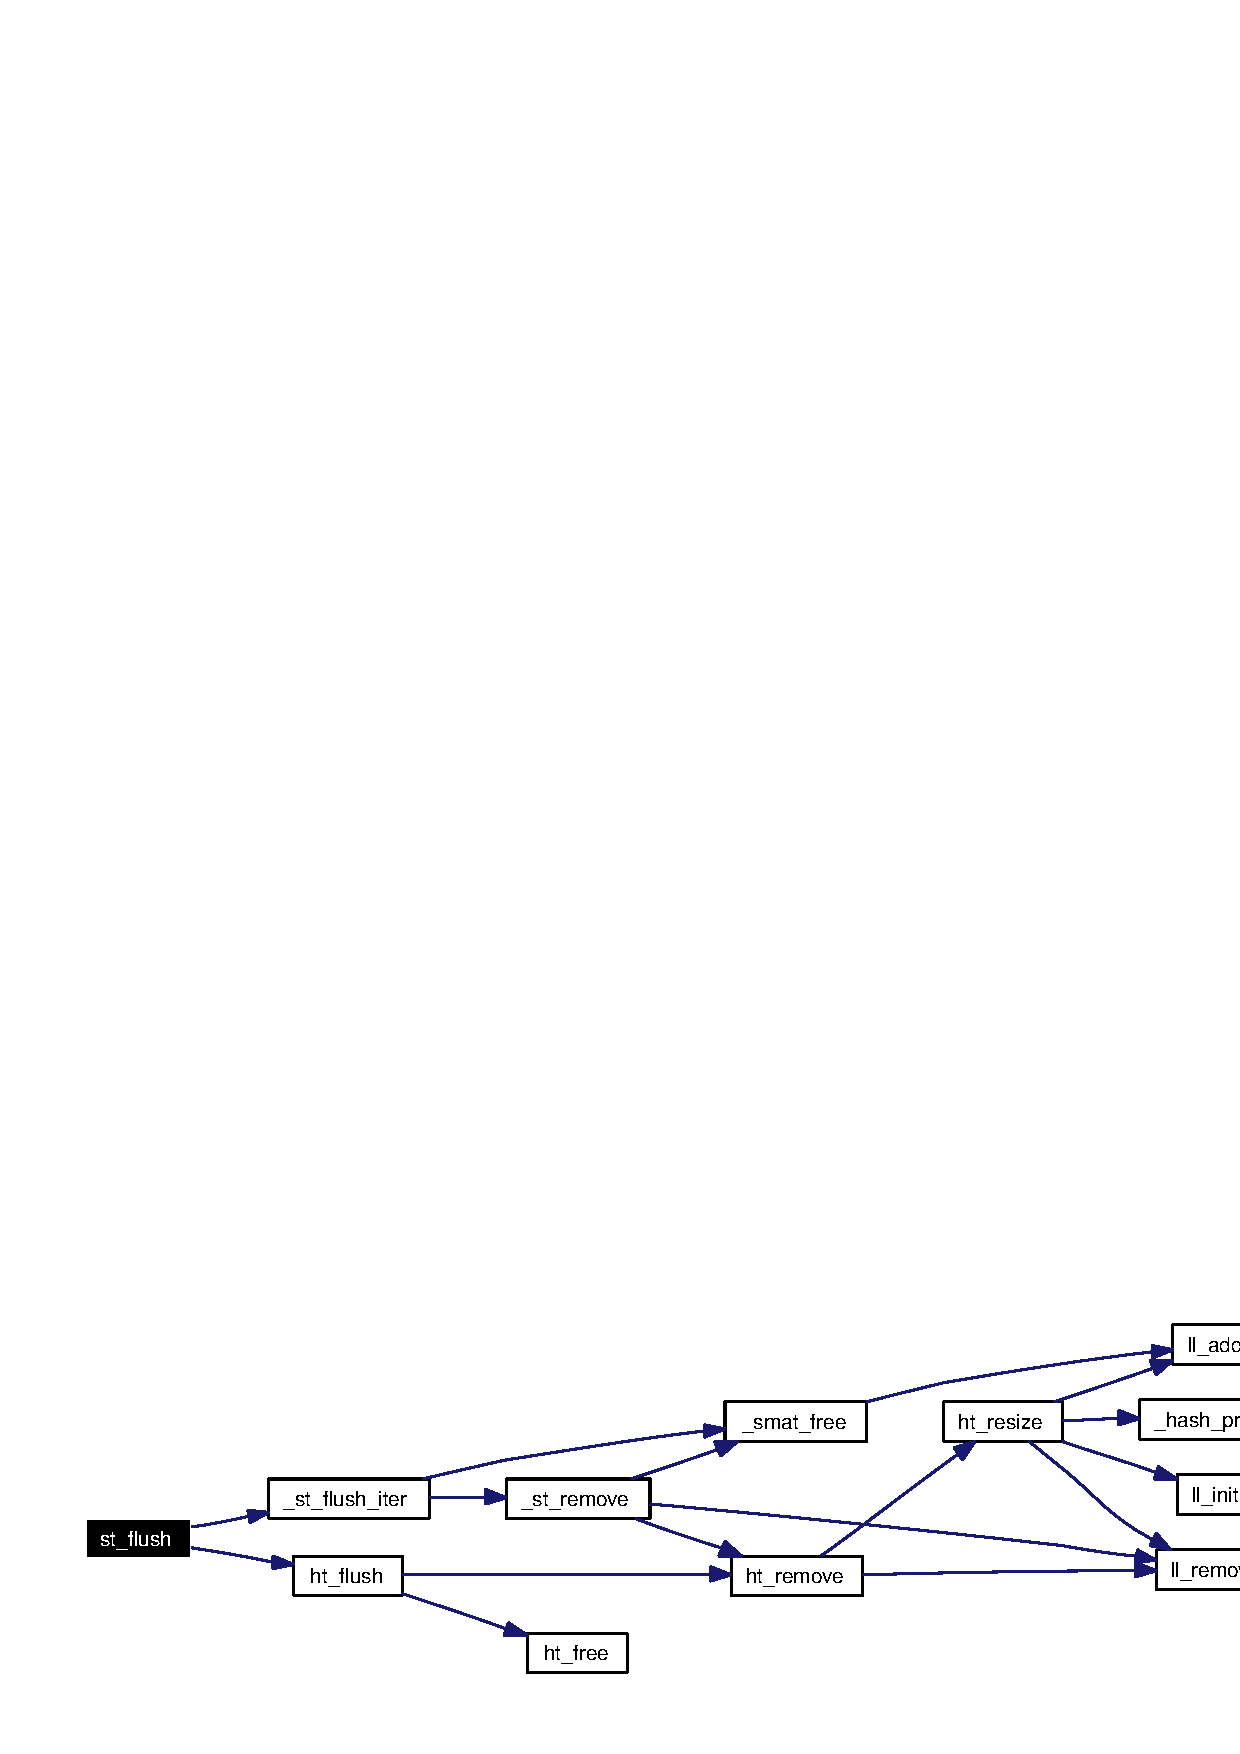
\includegraphics[width=313pt]{group__dbprim__smat_ga15_cgraph}
\end{center}
\end{figure}
\hypertarget{group__dbprim__smat_ga17}{
\index{dbprim_smat@{dbprim\_\-smat}!st_free@{st\_\-free}}
\index{st_free@{st\_\-free}!dbprim_smat@{dbprim\_\-smat}}
\subsubsection[st\_\-free]{\setlength{\rightskip}{0pt plus 5cm}unsigned long st\_\-free (\hyperlink{struct__smat__table__s}{smat\_\-table\_\-t} $\ast$ {\em table})}}
\label{group__dbprim__smat_ga17}


This function releases the memory used by the bucket table of the empty hash table associated with a sparse matrix.

\begin{Desc}
\item[Parameters:]
\begin{description}
\item[\mbox{$\leftarrow$} {\em table}]A pointer to a \hyperlink{group__dbprim__smat_ga0}{smat\_\-table\_\-t}.\end{description}
\end{Desc}
\begin{Desc}
\item[Return values:]
\begin{description}
\item[{\em DB\_\-ERR\_\-BADARGS}]An invalid argument was given. \item[{\em DB\_\-ERR\_\-FROZEN}]The table is frozen. \item[{\em DB\_\-ERR\_\-NOTEMPTY}]The table is not empty.\end{description}
\end{Desc}


Definition at line 34 of file st\_\-free.c.

References ht\_\-free(), \_\-smat\_\-table\_\-s::st\_\-table, and st\_\-verify.

Here is the call graph for this function:\begin{figure}[H]
\begin{center}
\leavevmode
\includegraphics[width=88pt]{group__dbprim__smat_ga17_cgraph}
\end{center}
\end{figure}
\hypertarget{group__dbprim__smat_ga10}{
\index{dbprim_smat@{dbprim\_\-smat}!st_init@{st\_\-init}}
\index{st_init@{st\_\-init}!dbprim_smat@{dbprim\_\-smat}}
\subsubsection[st\_\-init]{\setlength{\rightskip}{0pt plus 5cm}unsigned long st\_\-init (\hyperlink{struct__smat__table__s}{smat\_\-table\_\-t} $\ast$ {\em table}, unsigned long {\em flags}, \hyperlink{group__dbprim__smat_ga3}{smat\_\-resize\_\-t} {\em resize}, void $\ast$ {\em extra}, unsigned long {\em init\_\-mod})}}
\label{group__dbprim__smat_ga10}


This function initializes a sparse matrix table.

\begin{Desc}
\item[Parameters:]
\begin{description}
\item[\mbox{$\leftarrow$} {\em table}]A pointer to a \hyperlink{group__dbprim__smat_ga0}{smat\_\-table\_\-t} to be initialized. \item[\mbox{$\leftarrow$} {\em flags}]A bit-wise OR of \hyperlink{group__dbprim__hash_ga23}{HASH\_\-FLAG\_\-AUTOGROW} and \hyperlink{group__dbprim__hash_ga24}{HASH\_\-FLAG\_\-AUTOSHRINK}. If neither behavior is desired, use 0. \item[\mbox{$\leftarrow$} {\em resize}]A \hyperlink{group__dbprim__hash_ga6}{hash\_\-resize\_\-t} function pointer for determining whether resizing is permitted and/or for notification of the resize. \item[\mbox{$\leftarrow$} {\em extra}]Extra pointer data that should be associated with the sparse matrix table. \item[\mbox{$\leftarrow$} {\em init\_\-mod}]An initial modulus for the table. This will presumably be extracted by \hyperlink{group__dbprim__smat_ga37}{st\_\-modulus()} in a previous invocation of the application. A 0 value is valid.\end{description}
\end{Desc}
\begin{Desc}
\item[Return values:]
\begin{description}
\item[{\em DB\_\-ERR\_\-BADARGS}]An invalid argument was given. \item[{\em ENOMEM}]Unable to allocate memory.\end{description}
\end{Desc}


Definition at line 34 of file st\_\-init.c.

References \_\-smat\_\-resize(), hash\_\-comp(), hash\_\-fnv1a(), ht\_\-init(), SMAT\_\-TABLE\_\-MAGIC, \_\-smat\_\-table\_\-s::st\_\-extra, \_\-smat\_\-table\_\-s::st\_\-magic, \_\-smat\_\-table\_\-s::st\_\-resize, and \_\-smat\_\-table\_\-s::st\_\-table.

Here is the call graph for this function:\begin{figure}[H]
\begin{center}
\leavevmode
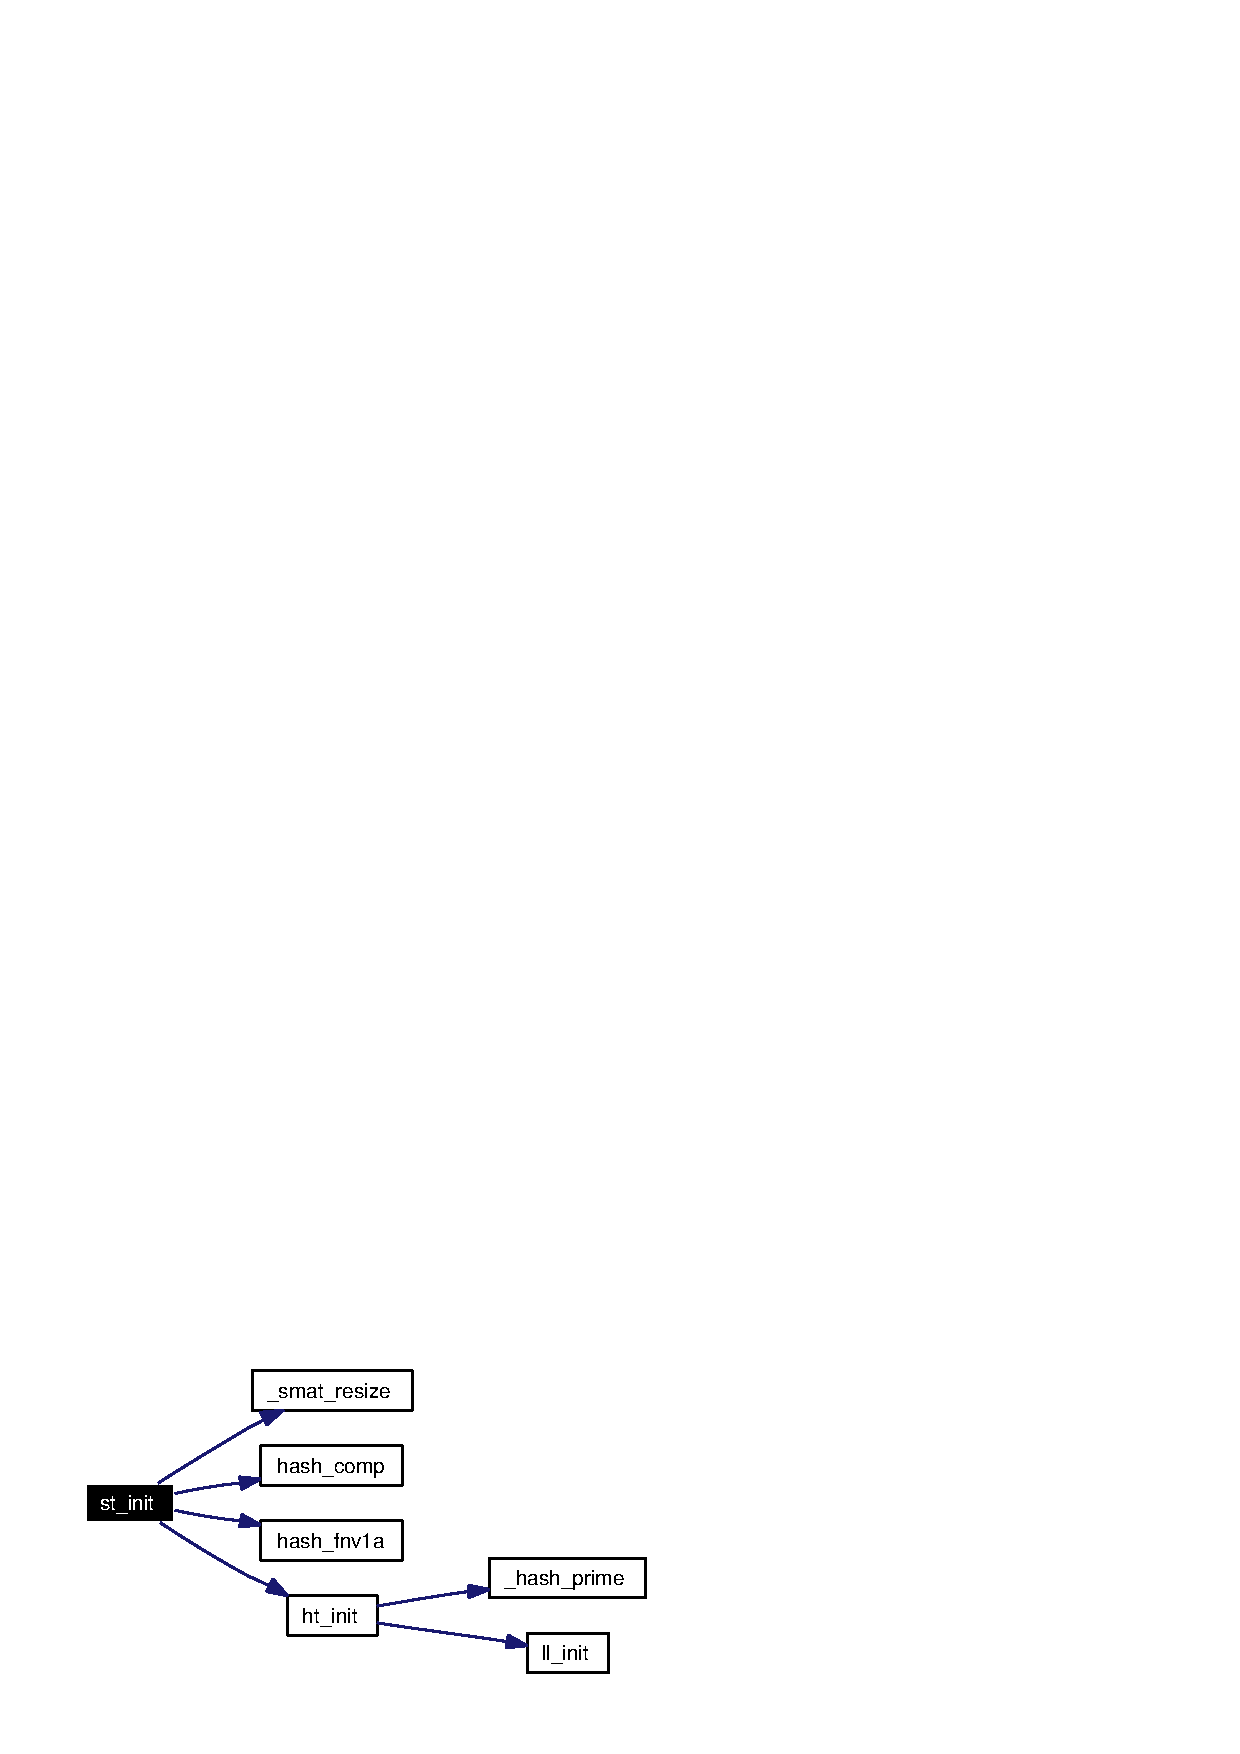
\includegraphics[width=157pt]{group__dbprim__smat_ga10_cgraph}
\end{center}
\end{figure}
\hypertarget{group__dbprim__smat_ga14}{
\index{dbprim_smat@{dbprim\_\-smat}!st_iter@{st\_\-iter}}
\index{st_iter@{st\_\-iter}!dbprim_smat@{dbprim\_\-smat}}
\subsubsection[st\_\-iter]{\setlength{\rightskip}{0pt plus 5cm}unsigned long st\_\-iter (\hyperlink{struct__smat__table__s}{smat\_\-table\_\-t} $\ast$ {\em table}, \hyperlink{group__dbprim__smat_ga4}{smat\_\-iter\_\-t} {\em iter\_\-func}, void $\ast$ {\em extra})}}
\label{group__dbprim__smat_ga14}


This function iterates over every entry in a sparse matrix (in an unspecified order), executing the given {\tt iter\_\-func} on each entry.

\begin{Desc}
\item[Parameters:]
\begin{description}
\item[\mbox{$\leftarrow$} {\em table}]A pointer to a \hyperlink{group__dbprim__smat_ga0}{smat\_\-table\_\-t}. \item[\mbox{$\leftarrow$} {\em iter\_\-func}]A pointer to a callback function used to perform user-specified actions on an entry in a sparse matrix. {\tt NULL} is an invalid value. See the documentation for \hyperlink{group__dbprim__smat_ga4}{smat\_\-iter\_\-t} for more information. \item[\mbox{$\leftarrow$} {\em extra}]A {\tt void} pointer that will be passed to {\tt iter\_\-func}.\end{description}
\end{Desc}
\begin{Desc}
\item[Return values:]
\begin{description}
\item[{\em DB\_\-ERR\_\-BADARGS}]An argument was invalid. \item[{\em DB\_\-ERR\_\-FROZEN}]The sparse matrix is frozen.\end{description}
\end{Desc}


Definition at line 77 of file st\_\-iter.c.

References \_\-st\_\-iter\_\-iter(), ht\_\-iter(), \_\-st\_\-iter\_\-s::si\_\-extra, \_\-st\_\-iter\_\-s::si\_\-iter, \_\-st\_\-iter\_\-s::si\_\-table, \_\-smat\_\-table\_\-s::st\_\-table, and st\_\-verify.

Here is the call graph for this function:\begin{figure}[H]
\begin{center}
\leavevmode
\includegraphics[width=97pt]{group__dbprim__smat_ga14_cgraph}
\end{center}
\end{figure}
\hypertarget{group__dbprim__smat_ga12}{
\index{dbprim_smat@{dbprim\_\-smat}!st_remove@{st\_\-remove}}
\index{st_remove@{st\_\-remove}!dbprim_smat@{dbprim\_\-smat}}
\subsubsection[st\_\-remove]{\setlength{\rightskip}{0pt plus 5cm}unsigned long st\_\-remove (\hyperlink{struct__smat__table__s}{smat\_\-table\_\-t} $\ast$ {\em table}, \hyperlink{struct__smat__entry__s}{smat\_\-entry\_\-t} $\ast$ {\em entry})}}
\label{group__dbprim__smat_ga12}


This function removes the given entry from the specified sparse matrix.

\begin{Desc}
\item[Parameters:]
\begin{description}
\item[\mbox{$\leftarrow$} {\em table}]A pointer to a \hyperlink{group__dbprim__smat_ga0}{smat\_\-table\_\-t}. \item[\mbox{$\leftarrow$} {\em entry}]A pointer to a \hyperlink{group__dbprim__smat_ga2}{smat\_\-entry\_\-t} to be removed from the table.\end{description}
\end{Desc}
\begin{Desc}
\item[Return values:]
\begin{description}
\item[{\em DB\_\-ERR\_\-BADARGS}]An invalid argument was given. \item[{\em DB\_\-ERR\_\-WRONGTABLE}]Entry is not in this sparse matrix. \item[{\em DB\_\-ERR\_\-UNRECOVERABLE}]An unrecoverable error occurred while removing the entry from the table.\end{description}
\end{Desc}


Definition at line 63 of file st\_\-remove.c.

References \_\-st\_\-remove(), \_\-smat\_\-entry\_\-s::se\_\-table, se\_\-verify, ST\_\-REM\_\-FIRST, ST\_\-REM\_\-FREE, ST\_\-REM\_\-HASH, ST\_\-REM\_\-SECOND, and st\_\-verify.

Here is the call graph for this function:\begin{figure}[H]
\begin{center}
\leavevmode
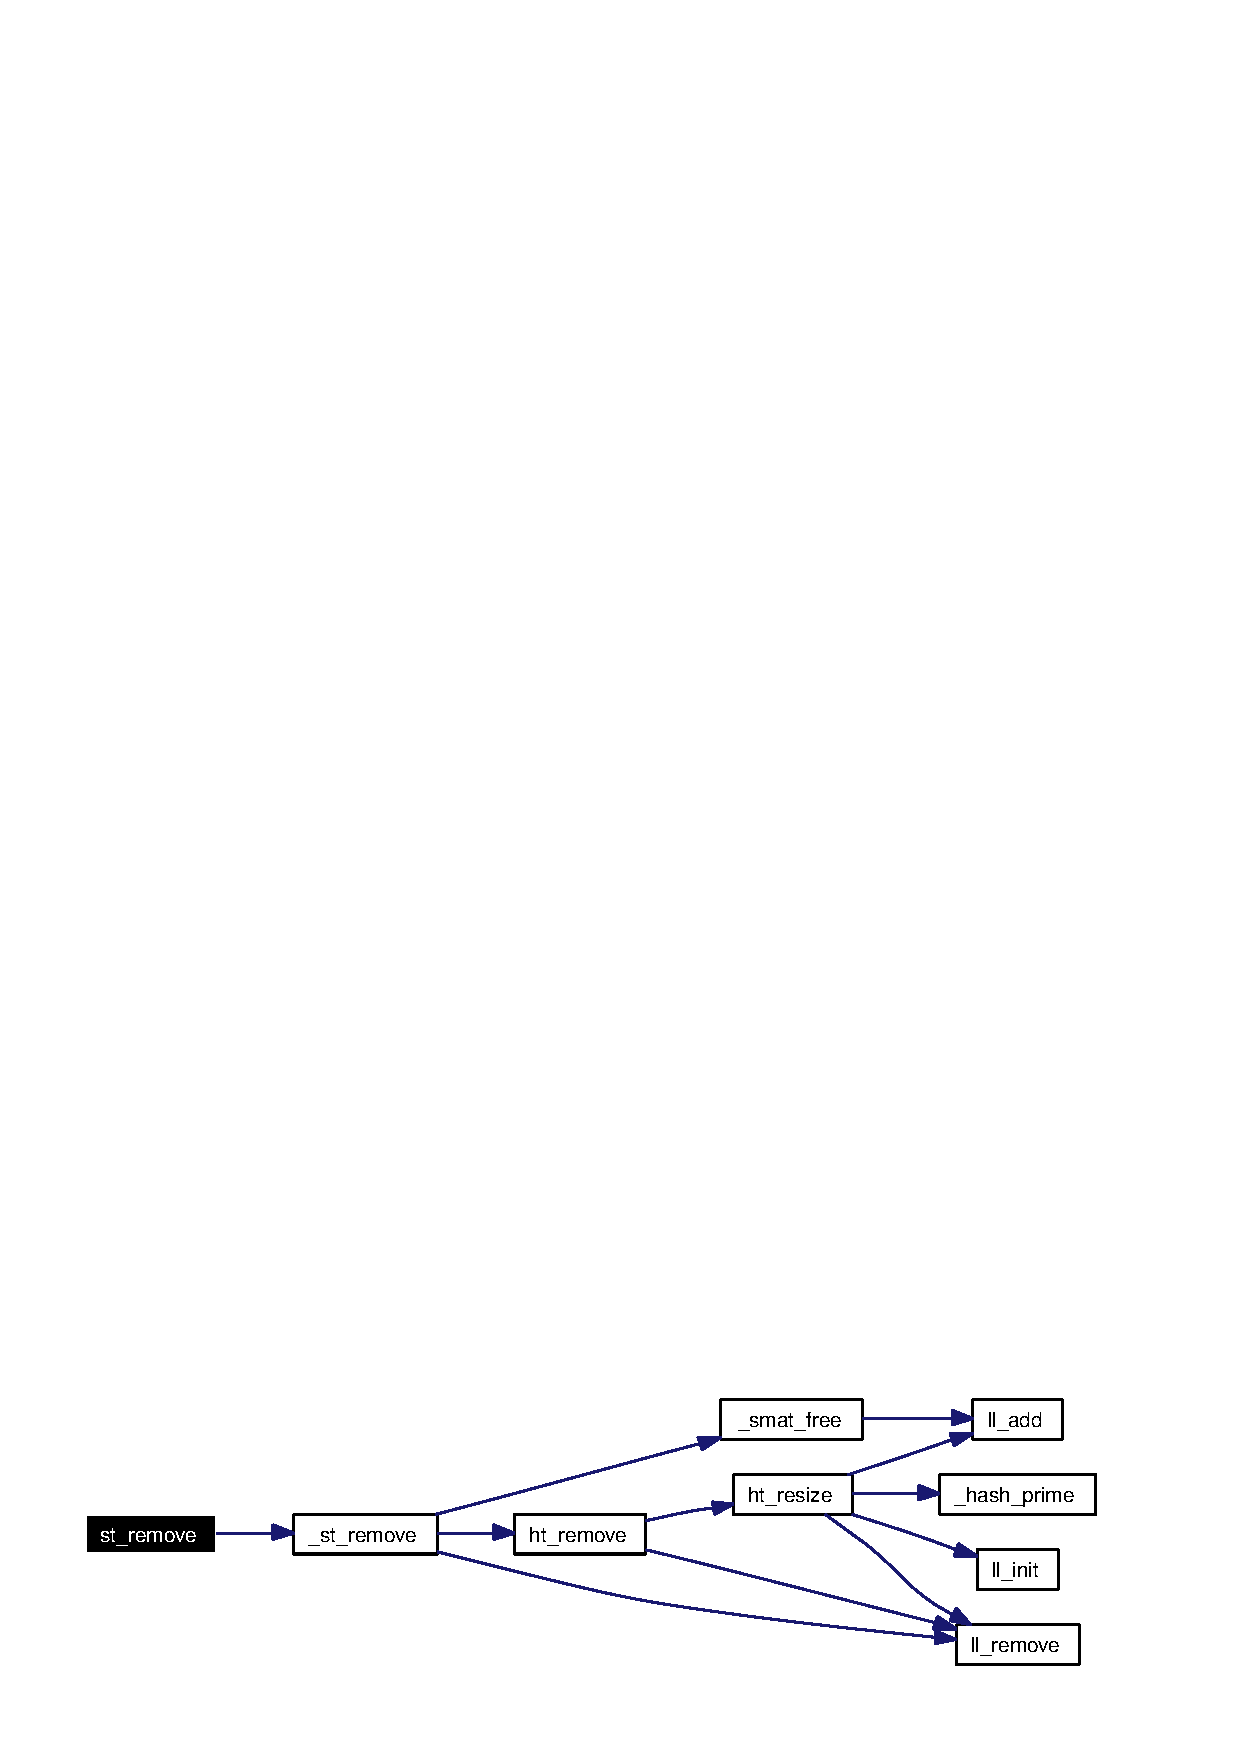
\includegraphics[width=265pt]{group__dbprim__smat_ga12_cgraph}
\end{center}
\end{figure}
\hypertarget{group__dbprim__smat_ga16}{
\index{dbprim_smat@{dbprim\_\-smat}!st_resize@{st\_\-resize}}
\index{st_resize@{st\_\-resize}!dbprim_smat@{dbprim\_\-smat}}
\subsubsection[st\_\-resize]{\setlength{\rightskip}{0pt plus 5cm}unsigned long st\_\-resize (\hyperlink{struct__smat__table__s}{smat\_\-table\_\-t} $\ast$ {\em table}, unsigned long {\em new\_\-size})}}
\label{group__dbprim__smat_ga16}


This function resizes the hash table associated with a sparse matrix based on the {\tt new\_\-size} parameter. See the documentation for \hyperlink{group__dbprim__hash_ga17}{ht\_\-resize()} for more information.

\begin{Desc}
\item[Parameters:]
\begin{description}
\item[\mbox{$\leftarrow$} {\em table}]A pointer to a \hyperlink{group__dbprim__smat_ga0}{smat\_\-table\_\-t}. \item[\mbox{$\leftarrow$} {\em new\_\-size}]A new size value for the table.\end{description}
\end{Desc}
\begin{Desc}
\item[Return values:]
\begin{description}
\item[{\em DB\_\-ERR\_\-BADARGS}]An argument was invalid. \item[{\em DB\_\-ERR\_\-FROZEN}]The table is currently frozen. \item[{\em DB\_\-ERR\_\-UNRECOVERABLE}]A catastrophic error was encountered. The table is now unusable. \item[{\em ENOMEM}]No memory could be allocated for the new bucket table.\end{description}
\end{Desc}


Definition at line 34 of file st\_\-resize.c.

References ht\_\-resize(), \_\-smat\_\-table\_\-s::st\_\-table, and st\_\-verify.

Here is the call graph for this function:\begin{figure}[H]
\begin{center}
\leavevmode
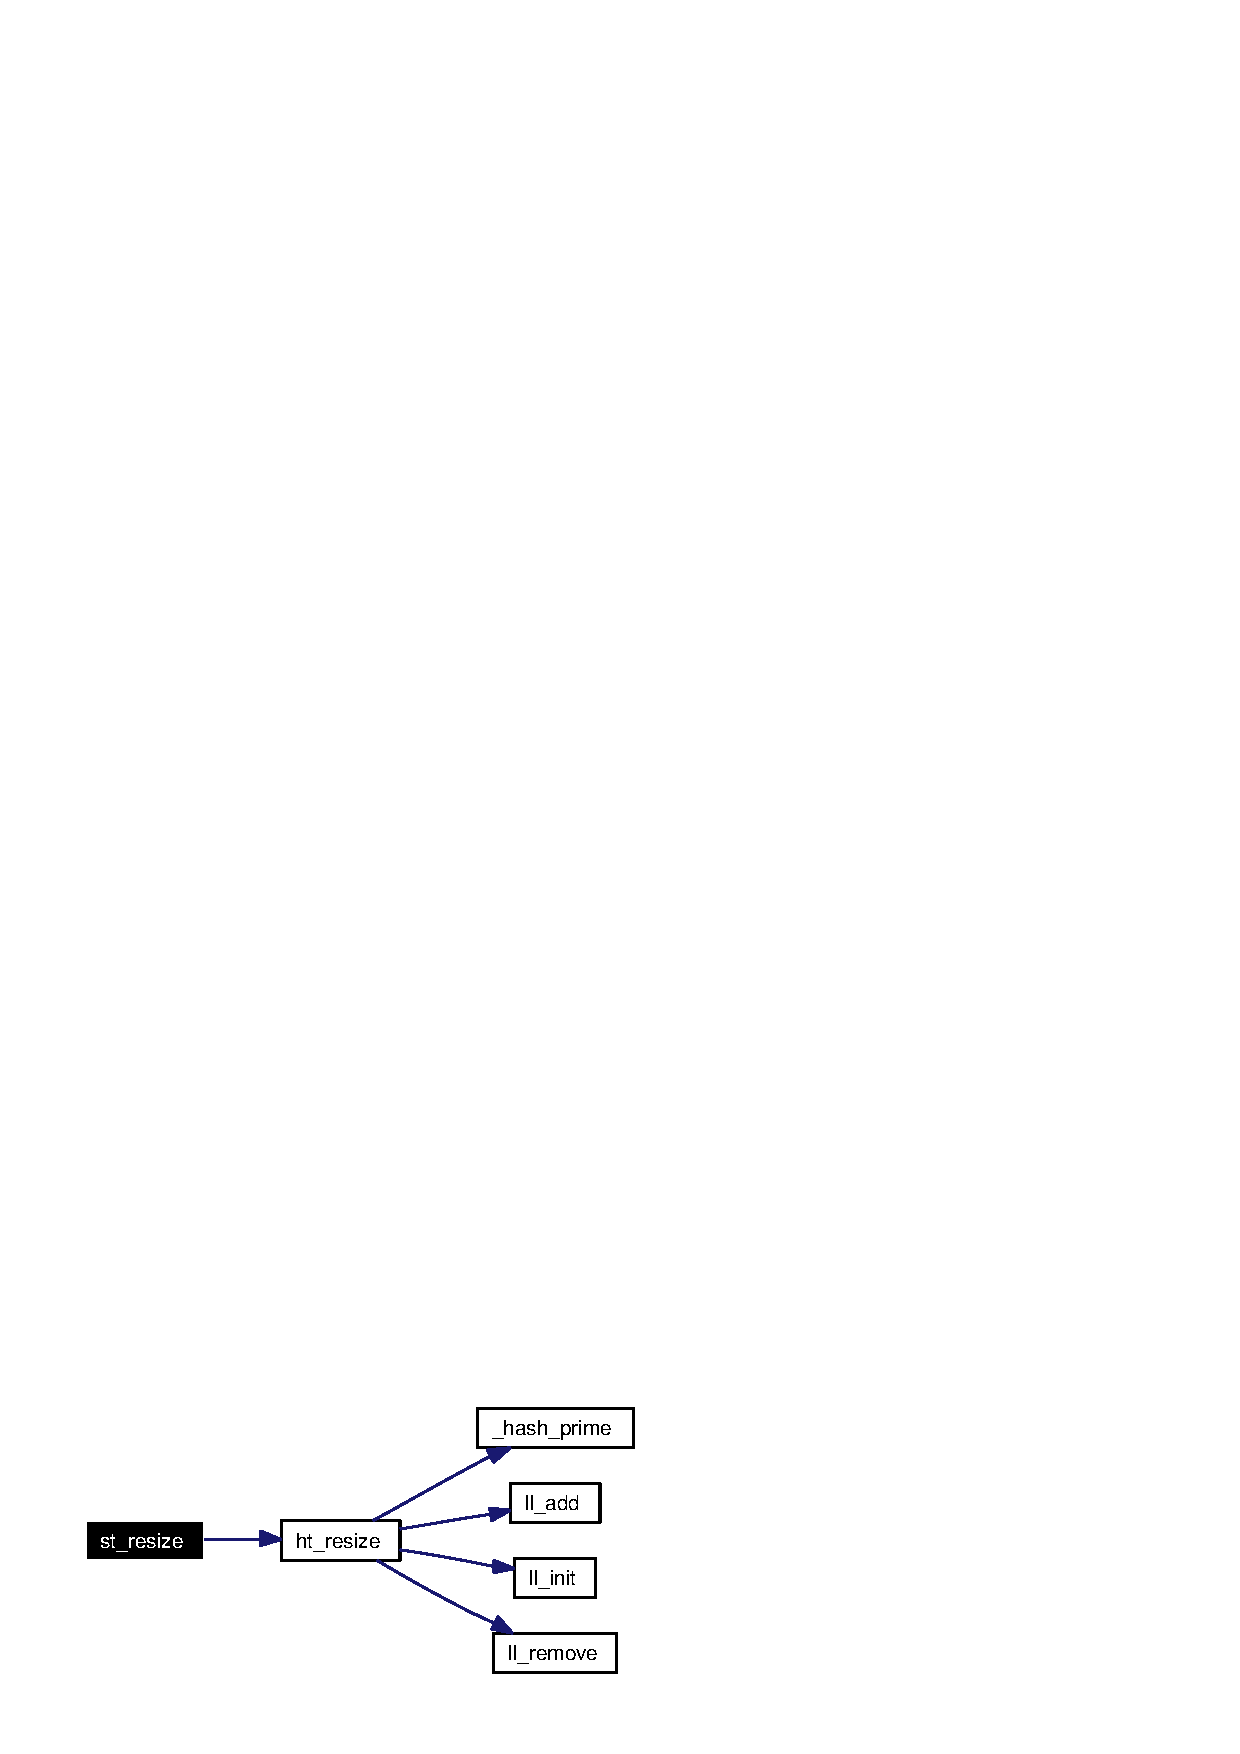
\includegraphics[width=154pt]{group__dbprim__smat_ga16_cgraph}
\end{center}
\end{figure}


\subsection{Variable Documentation}
\hypertarget{group__dbprim__smat_ga7}{
\index{dbprim_smat@{dbprim\_\-smat}!_smat_freelist@{\_\-smat\_\-freelist}}
\index{_smat_freelist@{\_\-smat\_\-freelist}!dbprim_smat@{dbprim\_\-smat}}
\subsubsection[\_\-smat\_\-freelist]{\setlength{\rightskip}{0pt plus 5cm}\hyperlink{struct__link__head__s}{link\_\-head\_\-t} \hyperlink{group__dbprim__smat_ga7}{\_\-smat\_\-freelist}\hspace{0.3cm}{\tt  \mbox{[}static\mbox{]}}}}
\label{group__dbprim__smat_ga7}


\begin{Desc}
\item[For internal use only.]
This variable is the head of a linked list of free \hyperlink{group__dbprim__smat_ga2}{smat\_\-entry\_\-t} structures.\end{Desc}


Definition at line 45 of file smat\_\-freelist.c.